%%%  کلاس AUTthesis، نسخه آبان 1397
%%%   دانشگاه صنعتی امیرکبیر                 http://www.aut.ac.ir
%%%  تالار گفتگوی پارسی‌لاتک،       http://forum.parsilatex.com
%%%   آپدیت شده در آبان 95
%%%   پشتیبانی و راهنمایی          badali_farhad@yahoo.com
%%%
%%%   بازبینی و اصلاح شده در آبان ماه 1397
%%%  Tested via TeXstudio in TeXlive 2014-2018.
%%%

%-----------------------------------------------------------------------------------------------------
%        روش اجرا.: 2 بار F1 ، 2 بار  F11(به منظور تولید مراجع) ، دوبار Ctrl+Alt+I (به منظور تولید نمایه) و دو بار F1 -------> مشاهده Pdf
%%%%%%%%%%%%%%%%%%%%%%%%%%%%%%%%%%%%%%%%%%%%%%%%%%%%%%
%   TeXstudio as your IDE
%%  برای compile در TeXstudio تنها کافی است منوی Options->Configure TeXstudio را زده و در پنجره Configure TeXstudio در بخش Build گزینه Default Compiler را به XeLaTeX تغییر دهید. سند شما به راحتی compile خواهد شد.
%   F1 & F5 : Build & view
%   F6      : Compile
%   F7      : View
%   --------------
%%%%%%%%%%%%%%%%%%%%%%%%%%%%%%%%%%%%%%%%%%%%%%%%%%%%%%
%        اگر قصد نوشتن رساله دکتری را دارید، در خط زیر به جای msc،
%      کلمه phd را قرار دهید. کلیه تنظیمات لازم، به طور خودکار، اعمال می‌شود.
%%% !TEX TS-program = XeLaTeX
\documentclass[oneside, openany, bsc, 12pt]{AUTthesis}
%       فایل commands.tex را حتماً به دقت مطالعه کنید؛ چون دستورات مربوط به فراخوانی بسته زی‌پرشین 
%       و دیگر بسته‌ها و ... در این فایل قرار دارد و بهتر است که با نحوه استفاده از آنها آشنا شوید. توجه شود برای نسخه نهایی پایان‌نامه حتماً hyperref را 
%        غیرفعال کنید.


% در این فایل، دستورها و تنظیمات مورد نیاز، آورده شده است.
%-------------------------------------------------------------------------------------------------------------------
% در ورژن جدید زی‌پرشین برای تایپ متن‌های ریاضی، این سه بسته، حتماً باید فراخوانی شود.
\usepackage{amsthm,amssymb,amsmath,amsfonts}
% بسته‌ای برای تنطیم حاشیه‌های بالا، پایین، چپ و راست صفحه
\usepackage[top=30mm, bottom=30mm, left=25mm, right=30mm]{geometry}
% بسته‌‌ای برای ظاهر شدن شکل‌ها و تصاویر متن
\usepackage{graphicx}
\usepackage{color}
%بسته‌ای برای تنظیم فاصله عمودی خط‌های متن
\usepackage{setspace}
\usepackage{titletoc}
\usepackage{tocloft}
%با فعال کردن بسته زیر فوت‌نوت‌ها در هر صفحه ریست می‌شوند. حالت پیش‌فرض آن ریست شدن در هر فصل می‌باشد.
%\usepackage[perpage]{footmisc}
\usepackage{enumitem}
\usepackage{caption}
%\usepackage{titlesec}
% بسته‌ و دستوراتی برای ایجاد لینک‌های رنگی با امکان جهش
\usepackage[pagebackref=false,colorlinks,linkcolor=blue,citecolor=red]{hyperref}
\usepackage[nameinlink]{cleveref}%capitalize,,noabbrev
% \usepackage{polyglossia}

% \setdefaultlanguage[numerals=maghrib]{persian}
% \setotherlanguage{english}

 \AtBeginDocument{%
    \crefname{equation}{برابری}{equations}%
    \crefname{chapter}{فصل}{chapters}%
    \crefname{section}{بخش}{sections}%
    \crefname{appendix}{پیوست}{appendices}%
    \crefname{enumi}{مورد}{items}%
    \crefname{footnote}{زیرنویس}{footnotes}%
    \crefname{figure}{شکل}{figures}%
    \crefname{table}{جدول}{tables}%
    \crefname{theorem}{قضیه}{theorems}%
    \crefname{lemma}{لم}{lemmas}%
    \crefname{corollary}{نتیجه}{corollaries}%
    \crefname{proposition}{گزاره}{propositions}%
    \crefname{definition}{تعریف}{definitions}%
    \crefname{result}{نتیجه}{results}%
    \crefname{example}{مثال}{examples}%
    \crefname{remark}{نکته}{remarks}%
    \crefname{note}{یادداشت}{notes}%
}
% چنانچه قصد پرینت گرفتن نوشته خود را دارید، خط بالا را غیرفعال و  از دستور زیر استفاده کنید چون در صورت استفاده از دستور زیر‌‌، 
% لینک‌ها به رنگ سیاه ظاهر خواهند شد که برای پرینت گرفتن، مناسب‌تر است
%\usepackage[pagebackref=false]{hyperref}
% بسته‌ لازم برای تنظیم سربرگ‌ها
\usepackage{fancyhdr}
% بسته‌ای برای ظاهر شدن «مراجع»  در فهرست مطالب
\usepackage[nottoc]{tocbibind}
% دستورات مربوط به ایجاد نمایه
\usepackage{makeidx,multicol}
\setlength{\columnsep}{1.5cm}

\usepackage[bottom]{footmisc}
\usepackage{float}
%%%%%%%%%%%%%%%%%%%%%%%%%%
\usepackage{verbatim}
\makeindex
\usepackage{sectsty}
% فراخوانی بسته زی‌پرشین و تعریف قلم فارسی و انگلیسی
\usepackage{xepersian}%[extrafootnotefeatures]
\SepMark{-}
%حتماً از تک لایو 2014 استفاده کنید.
% \setmainfont[
%  UprightFont={XB Niloofar.ttf}
%  BoldFont={XB NiloofarBd.ttf}, 
% %  ItalicFont={XB NiloofarIt.ttf},
% %  BoldItalicFont={XB NiloofarBdIt.ttf}
%  ]{}
% HERE
\usepackage[T1]{fontenc}
% \setmainfont[Path=fonts/,
%         UprightFont=XB Niloofar.ttf,
%         ItalicFont=XB NiloofarIt.ttf]
%   {XB Niloofar.ttf}
\settextfont[Scale=1]{XB Niloofar.ttf}
% \setlatintextfont{Times New Roman.ttf}
\renewcommand{\labelitemi}{$\bullet$}
%%%%%%%%%%%%%%%%%%%%%%%%%%
% چنانچه می‌خواهید اعداد در فرمول‌ها، انگلیسی باشد، خط زیر را غیرفعال کنید.
%در غیر اینصورت حتماً فونت PGaramond را نصب کنید.
% \setdigitfont[Scale=1.1]{Yas.ttf}%%Yas
\setcounter{secnumdepth}{4}
%%%%%%%%%%%%%%%%%%%%%%%%%%
% تعریف قلم‌های فارسی اضافی برای استفاده در بعضی از قسمت‌های متن
% \defpersianfont\nastaliq[Scale=2]{IranNastaliq.ttf}
% \defpersianfont\chapternumber[Scale=3]{B Nazanin.ttf}
%\chapterfont{\centering}%
%%%%%%%%%%%%%%%%%%%%%%%%%%
% دستوری برای تغییر نام کلمه «اثبات» به «برهان»
\renewcommand\proofname{\textbf{برهان}}

% دستوری برای تغییر نام کلمه «کتاب‌نامه» به «منابع و مراجع«
\renewcommand{\bibname}{منابع و مراجع}


% Headings for every page of ToC, LoF and Lot
\setlength{\cftbeforetoctitleskip}{-1.2em}
\setlength{\cftbeforelottitleskip}{-1.2em}
\setlength{\cftbeforeloftitleskip}{-1.2em}
\setlength{\cftaftertoctitleskip}{-1em}
\setlength{\cftafterlottitleskip}{-1em}
\setlength{\cftafterloftitleskip}{-1em}
%%\makeatletter
%%%%\renewcommand{\l@chapter}{\@dottedtocline{1}{1em\bfseries}{1em}}
%%%%\renewcommand{\l@section}{\@dottedtocline{2}{2em}{2em}}
%%%%\renewcommand{\l@subsection}{\@dottedtocline{3}{3em}{3em}}
%%%%\renewcommand{\l@subsubsection}{\@dottedtocline{4}{4em}{4em}}
%%%%\makeatother


\newcommand\tocheading{\par عنوان\hfill صفحه \par}
\newcommand\lofheading{\hspace*{.5cm}\figurename\hfill صفحه \par}
\newcommand\lotheading{\hspace*{.5cm}\tablename\hfill صفحه \par}

\renewcommand{\cftchapleader}{\cftdotfill{\cftdotsep}}
\renewcommand{\cfttoctitlefont}{\hspace*{\fill}\LARGE\bfseries}%\Large
\renewcommand{\cftaftertoctitle}{\hspace*{\fill}}
\renewcommand{\cftlottitlefont}{\hspace*{\fill}\LARGE\bfseries}%\Large
\renewcommand{\cftafterlottitle}{\hspace*{\fill}}
\renewcommand{\cftloftitlefont}{\hspace*{\fill}\LARGE\bfseries}
\renewcommand{\cftafterloftitle}{\hspace*{\fill}}

%%%%%%%%%%%%%%%%%%%%%%%%%%
% تعریف و نحوه ظاهر شدن عنوان قضیه‌ها، تعریف‌ها، مثال‌ها و ...
%برای شماره گذاری سه تایی قضیه ها
\theoremstyle{definition}
\newtheorem{definition}{تعریف}[section]
\newtheorem{remark}[definition]{نکته}
\newtheorem{note}[definition]{یادداشت}
\newtheorem{example}[definition]{نمونه}
\newtheorem{question}[definition]{سوال}
\newtheorem{remember}[definition]{یاداوری}
\theoremstyle{theorem}
\newtheorem{theorem}[definition]{قضیه}
\newtheorem{lemma}[definition]{لم}
\newtheorem{proposition}[definition]{گزاره}
\newtheorem{corollary}[definition]{نتیجه}
%%%%%%%%%%%%%%%%%%%%%%%%
%%%%%%%%%%%%%%%%%%%
%%% برای شماره گذاری چهارتایی قضیه ها و ...
%%\newtheorem{definition1}[subsubsection]{تعریف}
%%\newtheorem{theorem1}[subsubsection]{قضیه}
%%\newtheorem{lemma1}[subsubsection]{لم}
%%\newtheorem{proposition1}[subsubsection]{گزاره}
%%\newtheorem{corollary1}[subsubsection]{نتیجه}
%%\newtheorem{remark1}[subsubsection]{نکته}
%%\newtheorem{example1}[subsubsection]{مثال}
%%\newtheorem{question1}[subsubsection]{سوال}

%%%%%%%%%%%%%%%%%%%%%%%%%%%%

% دستورهایی برای سفارشی کردن صفحات اول فصل‌ها
\makeatletter
\newcommand\mycustomraggedright{%
 \if@RTL\raggedleft%
 \else\raggedright%
 \fi}
\def\@makechapterhead#1{%
\thispagestyle{style1}
\vspace*{20\p@}%
{\parindent \z@ \mycustomraggedright
\ifnum \c@secnumdepth >\m@ne
\if@mainmatter

\bfseries{\Huge \@chapapp}\small\space \chapternumber {\huge\thechapter}
\par\nobreak
\vskip 0\p@
\fi
\fi
\interlinepenalty\@M 
\Huge \bfseries #1\par\nobreak
\vskip 120\p@

}

\thispagestyle{empty}
\newpage}
\bidi@patchcmd{\@makechapterhead}{\thechapter}{\tartibi{chapter}}{}{}
\bidi@patchcmd{\chaptermark}{\thechapter}{\tartibi{chapter}}{}{}
\makeatother

\pagestyle{fancy}
\renewcommand{\chaptermark}[1]{\markboth{\chaptername~\tartibi{chapter}: #1}{}}

\fancypagestyle{style1}{
\fancyhf{} 
\fancyfoot[c]{\thepage}
\fancyhead[R]{\leftmark}%
\renewcommand{\headrulewidth}{1.2pt}
}


\fancypagestyle{style2}{
\fancyhf{}
\fancyhead[R]{چکیده}
\fancyfoot[C]{\thepage{}}
\renewcommand{\headrulewidth}{1.2pt}
}

\fancypagestyle{style3}{%
  \fancyhf{}%
  \fancyhead[R]{فهرست نمادها}
  \fancyfoot[C]{\thepage}%
  \renewcommand{\headrulewidth}{1.2pt}%
}

\fancypagestyle{style4}{%
  \fancyhf{}%
  \fancyhead[R]{فهرست جداول}
  \fancyfoot[C]{\thepage}%
  \renewcommand{\headrulewidth}{1.2pt}%
}

\fancypagestyle{style5}{%
  \fancyhf{}%
  \fancyhead[R]{فهرست اشکال}
  \fancyfoot[C]{\thepage}%
  \renewcommand{\headrulewidth}{1.2pt}%
}

\fancypagestyle{style6}{%
  \fancyhf{}%
  \fancyhead[R]{فهرست مطالب}
  \fancyfoot[C]{\thepage}%
  \renewcommand{\headrulewidth}{1.2pt}%
}

\fancypagestyle{style7}{%
  \fancyhf{}%
  \fancyhead[R]{نمایه}
  \fancyfoot[C]{\thepage}%
  \renewcommand{\headrulewidth}{1.2pt}%
}

\fancypagestyle{style8}{%
  \fancyhf{}%
  \fancyhead[R]{منابع و مراجع}
  \fancyfoot[C]{\thepage}%
  \renewcommand{\headrulewidth}{1.2pt}%
}
\fancypagestyle{style9}{%
  \fancyhf{}%
  \fancyhead[R]{واژه‌نامه‌ی فارسی به انگلیسی}
  \fancyfoot[C]{\thepage}%
  \renewcommand{\headrulewidth}{1.2pt}%
}

\fancypagestyle{style10}{%
  \fancyhf{}%
  \fancyhead[R]{فهرست معادلات}
  \fancyfoot[C]{\thepage}%
  \renewcommand{\headrulewidth}{1.2pt}%
}

%


%دستور حذف نام لیست تصاویر و لیست جداول از فهرست مطالب
\newcommand*{\BeginNoToc}{%
  \addtocontents{toc}{%
    \edef\protect\SavedTocDepth{\protect\the\protect\value{tocdepth}}%
  }%
  \addtocontents{toc}{%
    \protect\setcounter{tocdepth}{-10}%
  }%
}
\newcommand*{\EndNoToc}{%
  \addtocontents{toc}{%
    \protect\setcounter{tocdepth}{\protect\SavedTocDepth}%
  }%
}
\newcounter{savepage}
\renewcommand{\listfigurename}{فهرست اشکال}
\renewcommand{\listtablename}{فهرست جداول}

\newcommand{\listequationsname}{فهرست معادلات}
\newlistof{myequations}{equ}{\listequationsname}
\newcommand{\myequations}[1]{%
\addcontentsline{equ}{myequations}{\protect\numberline{\theequation}#1}\par}
\setlength{\cftmyequationsnumwidth}{2.5em}% Width of equation number in List of Equations


%\renewcommand\cftsecleader{\cftdotfill{\cftdotsep}}
%%%%%%%%%%%%%%%%%%%%%%%%%%%%%
%%%%%%%%%%%%%%%%%%%%%%%%%%%%
% \numberwithin{section}{equation}
\renewcommand{\theequation}{\arabic{section}.\arabic{equation}}
\newcommand{\hst}[]{\hspace{2mm}}
\newcommand{\hso}[]{\hspace{1mm}}

\begin{document}
\baselineskip=.75cm
\linespread{1.75}
%% -!TEX root = AUTthesis.tex
% در این فایل، عنوان پایان‌نامه، مشخصات خود، متن تقدیمی‌، ستایش، سپاس‌گزاری و چکیده پایان‌نامه را به فارسی، وارد کنید.
% توجه داشته باشید که جدول حاوی مشخصات پروژه/پایان‌نامه/رساله و همچنین، مشخصات داخل آن، به طور خودکار، درج می‌شود.
%%%%%%%%%%%%%%%%%%%%%%%%%%%%%%%%%%%%
% دانشکده، آموزشکده و یا پژوهشکده  خود را وارد کنید
\faculty{دانشکده مهندسی کامپیوتر}
% گرایش و گروه آموزشی خود را وارد کنید
\department{}
% عنوان پایان‌نامه را وارد کنید
\fatitle{توليد موسيقی با محاسبات کوانتومی}
% نام استاد(ان) راهنما را وارد کنید
\firstsupervisor{دکتر مرتضی صاحب‌الزمانی}
%\secondsupervisor{استاد راهنمای دوم}
% نام استاد(دان) مشاور را وارد کنید. چنانچه استاد مشاور ندارید، دستور پایین را غیرفعال کنید.
%\firstadvisor{دکتر بهادر بخشی}
%\secondadvisor{استاد مشاور دوم}
% نام نویسنده را وارد کنید
\name{عرفان }
% نام خانوادگی نویسنده را وارد کنید
\surname{عابدی}
%%%%%%%%%%%%%%%%%%%%%%%%%%%%%%%%%%
\thesisdate{مهر ۱۴۰۰}

% چکیده پایان‌نامه را وارد کنید
\fa-abstract{
امروزه، با نزدیک‌شدن تکنولوژی‌های ساخت سخت‌افزار به محدودیت‌های فیزیکی قانون مور
% \fnote{Moore's law}
و هم‌چنین، پیش‌رفت روزافزون تکنولوژی‌های فوق سرد
% \fnote{Cryogenics}
توجه بسیاری به دانشمندان به حوزه‌ی محاسبات کوانتومی معطوف شده است. 
کامپیوترهایی که در حال حاضر به صورت روزمره در حال استفاده هستند، در هنگام انجام محاسبات خود از قوانین فیزیک کلاسیک پیروی می‌کنند و به کامپیوترهای کلاسیک معروف هستند.
محاسباتی که توسط کامپیوترهای کوانتومی انجام می‌شوند، بر خلاف کامپیوترهای کلاسیک، تابع قوانین فیزیک کوانتومی هستند، و به همین علت، بسیاری بر این باور هستند که این گونه کامپیوترها در آینده‌ای نزدیک، قادر به انجام محاسباتی خواهند بود که به سادگی توسط کامپیوترهای کلاسیک ممکن نیست.
یادگیری ماشین کوانتومی
% \fnote{Quantum Machine Learning}
به گروهی از الگوریتم‌های کوانتومی اطلاق می‌شود که همانند یادگیری ماشین کلاسیک، تعدادی پارامتر قابل تنظیم دارند که بهینه‌سازی این پارامترها برای رسیدن به خروجی مطلوب، توسط یک کامپیوتر کلاسیک انجام می‌گیرد.
در عین حال، از همان روزهای اولیه‌ی پیدایش کامپیوترها، بسیاری به دنبال تولید ملودی‌های موسیقی با استفاده از قدرت پردازشی کامپیوترها بوده‌اند و تاکنون، الگوریتم‌های متعددی برای حصول این امر پیشنهاد شده اند.
در این پروژه، امکان تولید موسیقی با استفاده از الگوریتم‌های یادگیری ماشین کوانتومی بررسی شده و برنامه‌ی نرم‌افزاری‌ای برای انجام این کار توسعه داده شده است.
% در این پروژه، سعی شده با به کار گیری از یادگیری ماشین کوانتومی، ملودی‌های موسیقی بدیعی تولید شود.
}


% کلمات کلیدی پایان‌نامه را وارد کنید
\keywords{
محاسبات کوانتومی، یادگیری ماشین، تولید موسیقی کامپیوتری
}



\AUTtitle
%%%%%%%%%%%%%%%%%%%%%%%%%%%%%%%%%%
\vspace*{7cm}
\thispagestyle{empty}
\begin{center}

\includegraphics[height=5cm,width=12cm]{figures/besm.jpg}
\end{center}
% تاییدیه دفاع
\newpage
\thispagestyle{empty}
%\fontsize{18pt}{19pt}\selectfont

\section*{صفحه فرم ارزیابی و تصویب پایان نامه- فرم تأیید اعضاء كميته دفاع}

\captionsetup[figure]{list=no}

\begin{figure}[H]
	\centering
% 	\includegraphics[scale=0.8]{taeid}
\end{figure}

\captionsetup[figure]{list=yes}

%%%%%%%%%%%%%%%%%%%%%%%%%%%%%%%%%%%%%%%%%%%%%%%%%%%%%%%%%%%%%%%%%%%%%%%%%%%%%%%%%%%%%%%%%%%%%%%%%%
%%%%%%%%%%%%%%%%%%%%%%%%%%%%%%%%%%%%%%%%%%%%%%%%%%%%%%%%%%%%%%%%%%%%%%%%%%%%%%%%%%%%%%%%%%%%%%%%%%
\newpage
\thispagestyle{empty}
\begin{picture}(50,50)
  \put(17,0){
\includegraphics[scale=1.1]{figures/fa-logo.png}}
  \put(4.5,-13){\footnotesize{دانشگاه صنعتی امیرکبیر}}
  \put(10.5,-27){\footnotesize{(پلی‌تکنیک تهران)}}
  \put(170,30){\bf{به نام خدا}}
  \put(140,-5){\Large\bf{تعهدنامه اصالت اثر}}
  \put(310,0){تاریخ: \datethesis}
\end{picture}

\vspace*{2.5cm}

اين‌جانب {\bf{\fname\lname}} متعهد می‌شوم که مطالب مندرج در این پایان‌نامه حاصل کار پژوهشی این‌جانب، تحت نظارت و راهنمایی اساتید دانشگاه صنعتی امیرکبیر بوده و به دست‌آوردهای دیگران که در این پژوهش از آن‌ها استفاده شده است،
مطابق مقررات و روال متعارف ارجاع و در فهرست منابع و مآخذ ذکر گردیده است. این پایان‌نامه قبلاً برای احراز هیچ مدرک هم‌سطح یا بالاتر ارائه نگردیده است.

در صورت اثبات تخلف در هر زمان، مدرک تحصیلی صادر شده توسط دانشگاه از درجه اعتبار ساقط بوده و دانشگاه حق پی‌گیری قانونی خواهد داشت.


کلیه نتایج و حقوق حاصل از این پایان‌نامه متعلق به دانشگاه صنعتی امیرکبیر می‌باشد. هرگونه استفاده از نتایج علمی و عملی، واگذاری اطلاعات به دیگران یا چاپ و تکثیر، نسخه‌برداری، ترجمه و اقتباس از این پایان نامه بدون موافقت کتبی دانشگاه صنعتی امیرکبیر ممنوع است. 
نقل مطالب با ذکر منبع بلامانع است.\\
\vspace{2.5cm}


{\centerline {\bf{\fname\lname}}}
\vspace*{.2cm}
{\centerline{امضا}}
%%%%%%%%%%%%%%%%%%%%%%%%%%%%%%%%%
% چنانچه مایل به چاپ صفحات «تقدیم»، «نیایش» و «سپاس‌گزاری» در خروجی نیستید، خط‌های زیر را با گذاشتن ٪  در ابتدای آنها غیرفعال کنید.
% پایان‌نامه خود را تقدیم کنید
% نیایش خود را در فایل زیر بنویسید.
%%\begin{acknowledgementpage}

\vspace{1.5cm}

{\nastaliq
{
 نويسنده پايان‌نامه، درصورت تمايل ميتواند برای سپاسگزاری پايان‌نامه خود را به شخص يا اشخاص و يا ارگان خاصی تقدیم نماید.
}}\end{acknowledgementpage}
\newpage
% سپاسگزاری را در فایل زیر بنویسید.
%%%%%%%%%%%%%%%%%%%%%%%%%%%%%%%%%%%%
\newpage\thispagestyle{empty}
% سپاس‌گزاری
% {\nastaliq
سپاس‌گزاری
% }
\\[2cm]

این‌جانب،
\fullname
،
از استاد راهنمای خود، جناب آقای 
\ffirstsupervisor \space
به خاطر تمامی کمک‌ها و راهنمایی‌های سازنده‌شان در مسیر انجام این پروژه و نوشتن این گزارش سپاس‌گزارم.














% با استفاده از دستور زیر، امضای شما، به طور خودکار، درج می‌شود.
\signature








%%%%%%%%%%%%%%%%%%%%%%%%%%%%%%%%%%%%%%%%%
%%%%%%%%%%%%%%%%%%%%%%%%%%%%%%%%%کدهای زیر را تغییر ندهید.
\newpage\clearpage

\pagestyle{style2}

\vspace*{-1cm}
\section*{\centering چکیده}
%\addcontentsline{toc}{chapter}{چکیده}
\vspace*{.5cm}
\ffa-abstract
\vspace*{2cm}


{\noindent\large\textbf{واژه‌های کلیدی:}}\par
\vspace*{.5cm}
\fkeywords
% دستور زیر برای شماره گذاری صفحات قبل از فصل اول با حروف ابجد است.
\pagenumbering{alph}
%-----------------------------------------------------------------------------
% فایل زیر دستورات مربوط به نمایش صفحات فهرست مطالب- فهرست اشکال و جداول است.
%{\pagestyle{style2}
%\tableofcontents}\newpage
%
%\listoffigures
\cleardoublepage
%\addtocontents{toc}{\tocheading}
\pagestyle{style6}
\tableofcontents
\pagestyle{style6}
\cleardoublepage
%اگر لیست تصاویر و لیست جداول ندارید ، کدهای زیر را با گذاشتن % در ابتدای آنها، غیرفعال کنید.
\BeginNoToc
%============
\addtocontents{lof}{\lofheading}% add heading to the first page in LoF
\pagestyle{style10}
\listofmyequations
% \listoffigures
\thispagestyle{style10}
\clearpage

% \addtocontents{lof}{\lofheading}% add heading to the first page in LoF
\pagestyle{style5}
\listoffigures
\thispagestyle{style5}
\clearpage
%============
%\addtocontents{lot}{\lotheading}% add heading to the first page in LoT
%\thispagestyle{style4}
%\listoftables
%\thispagestyle{style4}
%============
%\cleardoublepage
%
%\cleardoublepage
%\setcounter{savepage}{\arabic{page}}
%\mainmatter
%\addtocontents{toc}{\tocheading}% add heading to the first page in ToC, after frontmatter entries
\EndNoToc
% در صورت تمایل می‌توانید با فعال کردن دستور بالا، لیست تصاویر را به  پایان‌نامه خود اضافه کنید.
%-------------------------------------------------------------------------symbols(فهرست نمادها)
% وجود لیست نمادها الزامیست.(لطفاً نمادهای خود را جایگذین نمادهای پیش‌فرض کنید.)
%%%%%%%%%%%%%%

{\centering\LARGE\textbf{فهرست نمادها}\par}%

\pagenumbering{alph}
\setcounter{page}{\thesavepage}
%\setcounter{page}{6}
\vspace*{1cm}

\pagestyle{style3}
%\thispagestyle{empty}
%\addcontentsline{toc}{chapter}{فهرست نمادها}
\symb{\text{ نماد}}{مفهوم}
\\
%مقادیر بالا را تغییر ندهید
%%%%%%%%%%%%%%%%%%%%%%%%%%%%%%%%%%%%%%%%%%%%%%%%%%%%%%%%%
\symb{\mathbb{R}^n}{
فضای اقلیدسی با بعد $n$
}
\symb{\mathbb{S}^n}{
کره یکه $n$ بعدی
}
\symb{M^m}{
خمینه $m$-بعدی $M$
}
\symb{\mathfrak{X}(M)}{
جبر میدان‌های  برداری هموار روی $M$
}
\symb{\mathfrak{X}^1(M)}{
مجموعه میدان‌های برداری هموار یکه روی $(M,g)$ 
}
\symb{\Omega^p(M)}{
مجموعه $p$-فرمی‌های روی خمینه $M$
}
\symb{Q}{
اپراتور ریچی
}
\symb{\mathcal{R}}{
تانسور انحنای ریمان
}
\symb{ric}{
تانسور ریچی
}
\symb{L}{
مشتق لی
}
\symb{\Phi}{
2-فرم اساسی خمینه تماسی
}
\symb{\nabla}{
التصاق لوی-چویتای
}
\symb{\Delta}{
لاپلاسین ناهموار
}
\symb{\nabla^*}{
عملگر خودالحاق صوری القا شده از التصاق لوی-چویتای
}
\symb{g_s}{
متر ساساکی
}
\symb{\nabla}{
التصاق لوی-چویتای وابسته به متر ساساکی
}
\symb{\Delta}{
عملگر لاپلاس-بلترامی روی $p$-فرم‌ها
}

%%%%%%%%%%%%%%%%%%%%%%%%%%%%%%%%%%%%%%%

\thispagestyle{style3}
\newpage
%\pagestyle{style1}
%%%%%%%%%%%%%%%%%%%%%%%%%%%%%%%%%%%%


\pagenumbering{arabic}
\pagestyle{style1}
%--------------------------------------------------------------------------chapters(فصل ها)

\chapter{مقدمه}

% \section{محاسبات کوانتومی}

با گذشت چهل سال از طرح ایده‌ی محاسبات کوانتومی توسط ریچارد فاینمن
\cite{feynman}،
توجه جهان به کامپیوترهای کوانتومی در بالاترین سطح خود قرار دارد
عمده‌ی این توجه پس از ابداع الگوریتم فاکتورگیری شور
\fnote{Shor's factorization algorithm}
و الگوریتم جست‌وجوی گروور 
\fnote{Grover's quantum search algorithm}
در دهه‌ی نود میلادی آغاز شده است. از آن روز تاکنون، تلاش‌های بسیار زیادی برای طراحی الگوریتم‌های جدید برای کاربردهای متنوع و دسترسی به برتری محاسباتی کوانتومی در حال انجام هستند. در زمان تحریر این گزارش، شرکت‌های بسیاری از جمله آی‌بی‌ام، مایکروسافت و گوگل در حال سرمایه‌گذاری‌های جدی بر روی ساخت کامپیوترهای کوانتومی هستند. به عنوان مثال، در سال ۲۰۱۹،
شرکت گوگل آزمایشی 
\cite{google_supremacy}
انجام داد که نشان‌گر برتری محاسباتی کوانتومی بود، به این معنا که پیچیدگی زمانی انجام این آزمایش در حالت کلاسیک بسیار بزرگ‌تر از حالت کوانتومی است.

با این وجود، به علت محدودیت تعداد کیوبیت\footnote{معادل کوانتومی یک بیت کلاسیک}
های کامپیوترهای کوانتومی فعلی، تلاش‌های اندکی در راستای تولید قطعات موسیقی با استفاده از الگوریتم‌های کوانتومی صورت گرفته‌است. دو الگوریتمی که تاکنون در این راستا تحت بررسی قرار گرفته‌اند، تولید موسیقی با استفاده از تولیدکننده‌ی اعداد تصادفی
و گشت گراف 
\cite{miranda}
بوده اند، اما به نظر می‌رسد به علت وجود معادلات موجی در فیزیک کوانتومی و این حقیقت که موسیقی در اصل تشکیل شده از موج‌های صوتی است، در آینده می‌توان ارتباطات خیلی بیش‌تری بین تولید موسیقی و محاسبات کوانتومی کشف کرد.

\newpage
\section{هدف پروژه}
% موضوع این پایان‌نامه، در گام نخست بررسی شیوه‌های موجود استفاده از الگوریتم‌های کوانتومی برای تولید موسیقی؛ و در گام دوم، معرفی دو شیوه جدید برای تولید موسیقی با استفاده از یادگیری ماشین کوانتومی است.
هدف این پروژه، طراحی نرم‌افزاری است که بتواند با استفاده از الگوریتم‌های موجود یادگیری ماشین کوانتومی و یک  مجموعه داده از برخی موسیقی‌های موجود، اقدام به تولید قطعه‌ی موسیقی
\fnote{Musical piece}
جدیدی کند.
مجموعه داده‌ی این پروژه به صورت سری گسسته‌ای از نت‌ها و آکوردهای موسیقی است که به صورت یک فایل 
\lr{midi}
ذخیره شده‌اند.
عمده‌ی نرم‌افزارهای پخش محتوای چندرسانه‌ای، قابلیت پخش موسیقی با استفاده از فایل‌های 
\lr{midi}
به عنوان ورودی را دارند، اما
 شایان ذکر است که این نوع ذخیره‌سازی، با ذخیره‌سازی‌های شناخته‌شده‌تر محتوای صوتی مانند فایل‌های 
 \lr{mp3}
 متفاوت است؛ چراکه فایل‌های
 \lr{mp3}
 با استفاده از پردازش سیگنال و تبدیل فوریه اقدام به ذخیره‌سازی می‌کنند.
 

\section{اجزاء پروژه} \label{sec:parts}
پیاده‌سازی این پروژه به‌صورت کلی شامل ۳ بخش می‌شود:
\begin{enumerate}
    \item ماژول
    \lr{Midi}
    که مسئولیت پردازش داده‌های موسیقی را بر عهده دارد. این ماژول تعدادی فایل که متشکل از چندین  را به صورتی که به عنوان ورودی برای الگوریتم کوانتومی به راحتی قابل استفاده باشند در می‌آورد. هم‌چنین، این ماژول پس از دریافت خروجی تولید شده به وسیله‌ی اجرای الگوریتم یادگیری ماشین کوانتومی بر روی ورودی‌ها، فایل قطعه‌ی موسیقی جدیدی را تولید می‌کند.
    \item ماژول
    \lr{QLSTM}
    که با استفاده از الگوریتم حافظه‌ی طولانی کوتاه-مدت کوانتومی
    \cite{chen_qlstm}
    ، اقدام به تولید قطعات موسیقی می‌کند.
    
    \item ماژول
    \lr{QuGAN}
    که با استفاده از الگوریتم شبکه‌ی زایای دشمن‌گونه کوانتومی
    \cite{lloyd_qugan} \cite{zoufal_qugan}
    ، اقدام به تولید قطعات موسیقی می‌کند.

\end{enumerate}

\section{ابزارهای مورد استفاده برای پیاده‌سازی}

برای پیاده‌سازی اجزای مختلف این پروژه، از چند کتاب‌خانه‌ی نرم‌افزاری استفاده شده که در فصول بعدی نقش آن‌ها به صورت کامل شرح داده خواهد شد، اما در این بخش صرفا به عنوان مقدمه از آن‌ها نام برده می‌شود:
\lr{
\begin{itemize}
	\item \lr{Music21}
	\item \lr{PyTorch}
	\item \lr{PennyLane}
\end{itemize}
}
\chapter{مفاهیم پایه}
در این فصل به معرفی مفاهیم پایه موردنیاز برای درک قسمت‌های مختلف پروژه و جزییات پیاده‌سازی آن پرداخته می‌شود.

\newcommand{\dd}[1]{\mathrm{d}#1}

% Quantum Computation

\section{محاسبات کوانتومی}

\subsection{سیستم‌های تک‌کیوبیتی}

طبق قوانین فیزیک کوانتومی، حالت یک سیستم می‌تواند به صورت ترکیب خطی‌ای از چند حالت پایه باشد، که این حالت‌های پایه، حالت‌هایی هستند که در قوانین فیزیک کلاسیک نیز حالات صحیحی برای توصیف سیستم هستند.
در محاسبات کوانتومی از بردارهای عمودی برای نشان‌دادن وضعیت یک سیستم استفاده می‌شود و وضعیت سیستم‌های چندکیوبیتی را نیز می‌توان از روی بردارهای یک سیستم تک‌کیوبیتی نیز ساخت.
\\
به طور معمول، در محاسبات کوانتومی، با سیستم‌هایی با تنها دو حالت پایه سر و کار داریم، به همین علت، بردارهای فضای حالات سیستم‌های تک‌کیوبیتی ۲ بعدی هستند. لذا دو بردار مستقل یکه به عنوان بردارهای پایه‌ی این فضا تعیین داده می‌شوند که رابطه‌ی ۱-به-۱ ای با حالات پایه‌ی بیت‌های کلاسیک دارند.
این حالات پایه به صورت زیر تعیین می‌شوند:
\begin{equation}
    |0\rangle = \begin{bmatrix} 1 \\ 0 \end{bmatrix} 
    \mspace{18mu}
    |1\rangle = \begin{bmatrix} 0 \\ 1 \end{bmatrix}
\end{equation} 
\myequations{بردارهای پایه تک‌کیوبیتی}

نشان دادن بردارهای حالت به صورت 
\lr{$|0\rangle$} و \lr{$|1\rangle$}
به نمادگذاری \lr{bra-ket} دیراک
\fnote{Dirac's bra-ket notation}
معروف است و به ازای هر
\lr{ket}
به صورت زیر:
\begin{equation}
    |\psi\rangle = \alpha |0\rangle + \beta |1\rangle
    = \begin{bmatrix}
    \alpha \\[3pt]
    \beta
    \end{bmatrix}
\end{equation}
یک \lr{bra}
به این صورت تعریف می‌شود:
\begin{equation}
    \langle \psi| = \alpha^* \langle0| + \beta^* \langle1| = \begin{bmatrix} \alpha^* & \beta^* \end{bmatrix} 
\end{equation}

که در این‌جا نماد \lr{$\alpha^*$}
به معنای مزدوج مخلط 
\fnote{Complex conjugate}
عدد \lr{$\alpha$}
است.
\newpage

حالت‌های سیستم در فیزیک کوانتومی در اکثر اوقات به صورت بردارهای مختلط بهنجار
\fnote{Normalizable}
نشان داده می‌شوند.
\begin{equation}
    |\psi\rangle = \alpha |0\rangle + \beta |1\rangle = \begin{bmatrix} \alpha \\ \beta \end{bmatrix} 
    ; \mspace{18mu}
    \alpha, \beta \in \mathbb{C}
\end{equation}
% \newpage
\myequations{فرم کلی بردار وضعیت سیستم تک کیوبیتی}
که به امر ایجاد یک بردار وضعیت از ترکیب خطی دو بردار وضعیت دیگر، اصل برهم‌نهی کوانتومی
\fnote{Quantum Superposition}
گفته می‌شود.

بهنجار بودن به معنای صدق شرایط زیر است:
\begin{equation}
    \alpha\alpha^* + \beta\beta^* = |\alpha|^2 + |\beta|^2 = 1
\end{equation}
\myequations{شرط بهنجار بودن}
% \newpage
\begin{figure}
	\centering
	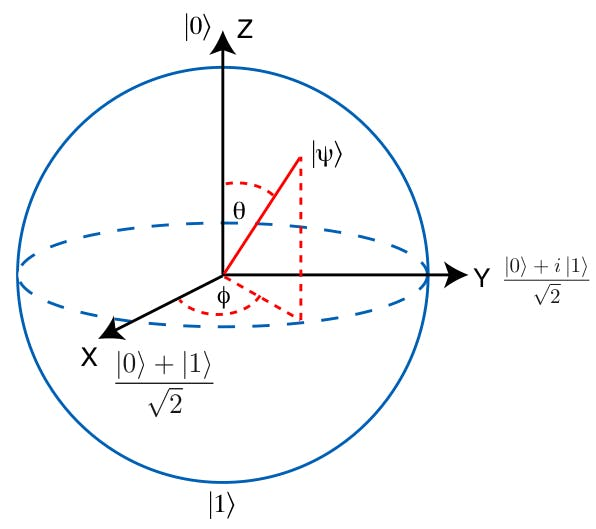
\includegraphics[scale=0.4]{figures/bloch.jpg}
	\caption{کره‌ی بلاخ}
	\label{fig:bloch}
\end{figure}
به علت شرط بهنجاری، می‌توان حالت کلی یک سیستم تک‌کیوبیتی را به صورت زیر نیز نوشت:
\begin{equation}
|\psi\rangle = \begin{bmatrix} e^{i\phi_1}\cos{\tfrac{\theta}{2}} \\[6pt] e^{i\phi_2}\sin{\tfrac{\theta}{2}} \end{bmatrix} 
\mspace{18mu}
\theta, \phi_1, \phi_2 \in {\rm I\!R}
\end{equation}
\myequations{حالت معادل فرم کلی بردار تک‌کیوبیتی}

که آن را می‌توان به صورت زیر نیز نوشت:
\begin{equation}
|\psi\rangle = e^{i\phi_1} \begin{bmatrix} \cos{\tfrac{\theta}{2}} \\[6pt] e^{i\phi_2-\phi_1}\sin{\tfrac{\theta}{2}} \end{bmatrix} = e^{i\phi_1} \begin{bmatrix} \cos{\tfrac{\theta}{2}} \\[6pt] e^{i\phi}\sin{\tfrac{\theta}{2}} \end{bmatrix}
\Rightarrow |\psi\rangle = \begin{bmatrix} \cos{\tfrac{\theta}{2}} \\[6pt] e^{i\phi}\sin{\tfrac{\theta}{2}} \end{bmatrix}
\end{equation}
\myequations{مهم نبودن فاز کلی سیستم}
در این معادله،
\lr{$\phi_1$}
 فاز کلی سیستم نامیده می‌شود که طبق قوانین فیزیک کوانتومی، در رفتار سیستم فاقد اهمیت است و به همین علت در مرحله‌ی آخر از آن صرف نظر شده‌است. \\
در نهایت، حالت کلی یک کیوبیت را می‌توان با استفاده از ابزاری به نام کره‌ی بلاخ (شکل
\ref{fig:bloch})
نمایش داد.

\subsection{سیستم‌های چندکیوبیتی}
اگر دو سیستم تک‌کیوبیتی جداگانه داشته باشیم، می‌توانیم آن‌ها را به صورت مجزا به صورت زیر تعریف می‌کنیم:
\begin{equation}
|a\rangle = \begin{bmatrix} a_0 \\ a_1 \end{bmatrix}, \quad |b\rangle = \begin{bmatrix} b_0 \\ b_1 \end{bmatrix}
\end{equation}
\myequations{دو کیوبیت مجزا}
در عین حال، می‌توانیم بردار وضعیت آن‌ها را به صورت هم‌زمان با استفاده از عملگری به نام ضرب تانسوری
\fnote{Tensor product}
تعریف کنیم که به صورت زیر عمل می‌کند:
\begin{equation}
|b\rangle \otimes |a\rangle = \begin{bmatrix} b_0 \times \begin{bmatrix} a_0 \\ a_1 \end{bmatrix} \\[12pt] b_1 \times \begin{bmatrix} a_0 \\ a_1 \end{bmatrix} \end{bmatrix} = \begin{bmatrix} b_0 a_0 \\[2pt] b_0 a_1 \\[2pt] b_1 a_0 \\[2pt] b_1 a_1 \end{bmatrix} = |ba\rangle
\end{equation}
\myequations{ضرب تانسوری}

\subsection{درهم‌تنیدگی}

درهم‌تنیدگی کوانتومی\fnote{Quantum Entanglement}
، یکی از اصول فیزیک کوانتومی است و به این معناست که برخی بردار وضعیت‌های سیستم‌های چندکیوبیتی را نمی‌توان به صورت ضرب تانسوری دو بردار تک‌کیوبیتی مجزا تعریف کرد. این امر نشان‌گر این است که وضعیت این دو کیوبیت به هم وابسته هستند.
به عنوان مثال، اگر بردارهای زیر که در محاسبات کوانتومی به وضعیت‌های بل 
\fnote{Bell states}
معروف هستند را در نظر بگیریم:
\begin{equation}
|{\Phi_\pm}\rangle = \frac{1}{\sqrt 2}\big(|0\rangle| 0\rangle\pm |1\rangle| 1\rangle\big), \qquad |{\Psi_{\pm}}\rangle=\frac{1}{\sqrt 2}\big(|0\rangle| 1\rangle\pm  |1\rangle|0\rangle\big)
\end{equation}
\myequations{بردار وضعیت‌های بل}

مشاهده می‌کنیم که هیچ‌کدام از این بردارها را نمی‌توان به صورت ضرب تانسوری‌ای از ترکیب خطی بردارهای
\lr{$|0\rangle$} و \lr{$|1\rangle$}
نوشت.

\subsection{گیت‌های کوانتومی}
در کامپیوترهای کلاسیک، محاسبات با استفاده از گیت‌هایی همانند 
\lr{AND}، \lr{OR} و NOT
انجام می‌شود.
معادل این گیت‌ها در محاسبات کوانتومی، گیت‌های کوانتومی هستند. این گیت‌ها به فرم ماتریس‌های یکانی 
\fnote{Unitary matrix}
\lr{$2^n \times 2^n$}
هستند که در این‌جا، عدد \lr{$n$}
نشان‌گر تعداد کیوبیت‌های سیستم است.

\subsubsection{
    گیت‌های کوانتومی تک‌کیوبیتی
}
در این بخش، صرفا تعدادی از گیت‌های کوانتومی به صورت خلاصه معرفی می‌شوند و اثر آن‌ها بر روی پایه‌های برداری فضای سیستم‌های تک‌کیوبیتی نشان داده می‌شود؛ چراکه تاثیر این گیت‌ها بر بردار وضعیت کیوبیت‌های دل‌خواه، با استفاده از ترکیب خطی تاثیر این گیت‌ها بر پایه‌های برداری به دست می‌آید.
\begin{equation}
X = \begin{bmatrix} 0 & 1 \\ 1 & 0 \end{bmatrix} \qquad
Y = \begin{bmatrix} 0 & -i \\ i & 0 \end{bmatrix} \qquad
Z = \begin{bmatrix} 1 & 0 \\ 0 & -1 \end{bmatrix} \qquad
H = \frac{1}{\sqrt{2}} \begin{bmatrix} 1 & 1 \\ 1 & -1 \end{bmatrix}
\end{equation}
\myequations{گیت‌های پائولی و هادامارد}
تمامی گیت‌های تک‌کیوبیتی، حالت خاصی از گیت پارامتردار 
\lr{$U_3$}
هستند.

\begin{equation}
U_3(\theta, \phi, \lambda) = \begin{bmatrix} \cos(\frac{\theta}{2}) & -e^{i\lambda}\sin(\frac{\theta}{2}) \\[6pt]
            e^{i\phi}\sin(\frac{\theta}{2}) & e^{i(\phi+\lambda)}\cos(\frac{\theta}{2})
     \end{bmatrix}
\end{equation}
\myequations{گیت \lr{$U_3$}}

\subsubsection{
    گیت‌های کوانتومی چند‌کیوبیتی
}
گیت‌های چندکیوبیتی نیز، همانند بردارهای وضعیت سیستم‌های چندکیوبیتی، دو نوع متفاوت دارند. در این بخش -برای سادگی محاسبات- تنها گیت‌های دوکیوبیتی را بررسی می‌کنیم؛ اما همین روابط برای تعداد کیوبیت‌های بالاتر نیز صادق است. \\
نوع اول، گیت‌هایی هستند که می‌توان آن‌ها را به صورت ضرب تانسوری دو گیت تک‌کیوبیتی تجزیه کرد.
\\
به عنوان مثال داریم:
\begin{equation}
    \begin{bmatrix}
    0 & 1 & 0 & 0 \\[3pt]
    1 & 0 & 0 & 0 \\[3pt]
    0 & 0 & 0 & 1 \\[3pt]
    0 & 0 & 1 & 0 
    \end{bmatrix} =
    \begin{bmatrix}
    1 & 0 \\[3pt]
    0 & 1 
    \end{bmatrix} \otimes
    \begin{bmatrix}
    0 & 1 \\[3pt]
    1 & 0
    \end{bmatrix}
    = \mathbb{I} \otimes X
\end{equation}
\myequations{گیت چندکیوبیتی ترکیبی}
این گیت معادل این امر است که هم‌زمان یک گیت همانی یا
$\mathbb{I}$
بر روی کیوبیت اول و یک گیت
$X$
بر روی کیوبیت دوم اعمال شود.

نوع دوم، گیت‌هایی هستند که به ضرب تانسوری دو گیت تک‌کیوبیتی تجزیه‌پذیر نیستند و تنها همین نوع گیت‌ها هستند که در هنگام اعمال بر روی برخی از حالت‌های کیوبیتی برهم‌نهیده، منجر به ایجاد درهم‌تنیدگی می‌شوند، به عنوان مثال، گیت
$CNOT$
\fnote{Controlled NOT}
به این صورت تعریف می‌شود:
\begin{equation}
    CNOT = \begin{bmatrix}
    1 & 0 & 0 & 0 \\[3pt]
    0 & 1 & 0 & 0 \\[3pt]
    0 & 0 & 0 & 1 \\[3pt]
    0 & 0 & 1 & 0 
    \end{bmatrix}
\end{equation}
\myequations{گیت CNOT}

و داریم:
\begin{equation}
    CNOT(H\otimes\bbmath{I}(|00\rangle)) = CNOT(\frac{1}{\sqrt{2}} \big( |0\rangle + |1\rangle \big) \otimes |0\rangle ) = \frac{1}{\sqrt{2}} (|00\rangle + |11\rangle)
\end{equation}
\myequations{تاثیر گیت \lr{CNOT} در ایجاد درهم‌تنیدگی}
این گیت به این دلیل نام‌گذاری شده که تاثیر آن بر روی کیوبیت دوم، توسط وضعیت کیوبیت اول کنترل شده؛ به این معنا که تنها در صورتی که کیوبیت اول در وضعیت
$|1\rangle$
باشد، گیت 
$X$
بر روی کیوبیت دوم اعمال خواهد شد.

\subsection{اندازه‌گیری}
اندازه‌گیری در محاسبات کوانتومی را می‌توان به گونه‌های مختلفی تعریف کرد، در این متن، یکی از این شیوه‌ها به عنوان معیار در نظر گرفته شده و تنها به آن پرداخته می‌شود.
عمل اندازه‌گیری در فیزیک کوانتومی، یک بردار وضعیت (که ممکن است برهم‌نهیده باشد) را ورودی گرفته و یک عدد حقیقی بین
$0$
و
$1$
را خروجی می‌دهد.
این اندازه‌گیری‌ها با توجه به یک مشاهده‌پذیر 
\fnote{Observable}
انجام می‌گیرند. مشاهده‌پذیرها در فیزیک کوانتومی، ماتریس‌های هرمیتی
\fnote{Hermitian matrix}
هستند. در این متن، فرض می‌شود که همیشه اندازه‌گیری با توجه به مشاهده‌پذیر 
$Z$
انجام می‌شود و به صورت زیر تعریف می‌شود:
\begin{equation}
    \langle \psi| Z^{\otimes n} | \psi\rangle
\end{equation}
\myequations{تعریف اندازه‌گیری}
که
$n$
تعداد کیوبیت‌های سیستم است. به عنوان مثال داریم:
\begin{equation}
    \langle 1 | Z | 1 \rangle = 
    \begin{bmatrix}
    0 & 1
    \end{bmatrix} 
    \begin{bmatrix}
    1 & 0 \\[3pt]
    0 & -1 \\[3pt]
    \end{bmatrix}
    \begin{bmatrix}
    0 \\[3pt] 1
    \end{bmatrix} 
    = \begin{bmatrix}
    0 & 1
    \end{bmatrix} 
    \begin{bmatrix}
    0 \\[3pt] -1
    \end{bmatrix}
    = -1
\end{equation}
\myequations{مثال اندازه‌گیری}
که معادل قرار گرفتن وضعیت کیوبیت بعد از اندازه‌گیری در حالت 
$|1\rangle$
خواهد بود. در صورتی که بردار موردنظر دچار برهم‌نهی باشد، خروجی اندازه‌گیری را امیدریاضی اندازه‌گیری‌های متعدد در نظر گرفته می‌شود..

در صورتی که این اندازه‌گیری‌ها به صورت جداگانه بر روی کیوبیت‌های سیستم اعمال شوند و در سیستم در‌هم‌تنیدگی وجود داشته‌باشد؛ درایه‌های آرایه‌ای که از این اندازه‌گیری‌ها به وجود می‌آید به میزان درهم‌تنیدگی موجود در سیستم با هم مرتبط خواهند بود. به عنوان مثال، اگر در سیستم
$\frac{1}{\sqrt{2}} (|00\rangle + |11\rangle)$
کیوبیت اول اندازه‌گیری شود و بعد از اندازه‌گیری در حالت 
$|0\rangle$
قرار بگیرد، کیوبیت دوم نیز حتما در حالت
$|0\rangle$
خواهد بود و بالعکس.

\section{یادگیری ماشین}
\chapter{کارهای پیشین}

\section{الگوریتم‌های کلاسیک تولید موسیقی}

از همان ابتدای پیدایش کامپیوترهای امروزی، موسیقی‌دان‌ها در تلاش برای تولید ملودی‌های جدید به وسیله‌ی کامپیوترها بوده‌اند.
مثال‌هایی از تلاش‌ها برای تولید موسیقی به وسیله‌ی محاسبات کلاسیک در زیر آمده‌اند:

\begin{itemize}
    \item 
    در دهه‌ی ۴۰ میلادی، پژوهشگران مجمع علمی-صنعتی استرالیا
\fnote{Australian council for scientific and industrial research (CSIR)}
بلندگویی را به یک کامپیوتر ام‌کا۱
\fnote{MK1}
متصل کردند تا صدایی که کامپیوتر در حین اجرای برنامه‌ها تولید می‌کرد را بشنوند. در همین راستا و در سال ۱۹۵۱، جف هیل
\fnote{Geoff Hill}
که ریاضی‌دانی با پیش‌زمینه‌ای در موسیقی بود، برنامه‌ای بر روی این کامپیوتر اجرا کرد تا صدای تولید شده تا حد بسیار خوبی شبیه ملودی‌های موسیقی شود.
\cite{CSIR_music}

\item
مدل‌های ترجمه‌ای
\fnote{Translational models}
سعی می‌کنند تا داده‌های غیرصوتی را به صوت تبدیل کنند؛ به عنوان مثال اگر مدلی ساخته شود که سعی کند عکس‌های با فرمت 
\lr{jpg}
را به فایل‌هایی با فرمت
\lr{mp3}
تبدیل کند (چرا که هر دوی این فرمت‌ها برای ذخیره‌سازی، از تبدیل فوریه استفاده می‌کنند)؛ ممکن است عکس یک خط صاف را به عنوان یک موسیقی با یک نت ثابت تعبیر کند

\item
مدل‌های گرامری
\fnote{Grammatical models}
سعی می‌کنند با پردازش کردن داده‌های موسیقیایی به عنوان جملات زبانی که همانند زبان طبیعی، از قواعد گرامری خاصی تبعیت می‌کند؛ الگوریتم‌های پردازش زبان طبیعی
\fnote{Natural Language Processing (NLP)}
را بر روی داده‌های موسیقیایی اعمال کنند.

\item
متدهای تکاملی، با استفاده از چهارچوب الگوریتم‌های ژنتیک
\fnote{Genetic algorithms}
؛ با یک سری از نت‌های موسیقی به عنوان ژن افراد یک جمعیت برخورد می‌کنند و بعد از ترکیب کردن ژن‌های این افراد و ایجاد جهش‌های تصادفی در این ژن‌ها، موسیقی‌های جدیدی تولید کنند.
به عنوان مثال، یک الگوریتم ژنتیک ممکن است دو گام زیر را به این صورت ترکیب کند:
\begin{equation}
\begin{gathered}
    C_{major} = [C, D, E, F, G, A, B, C]\\[3pt]
    A_{major} = [A, B, C\sharp, D, E, F\sharp, G\sharp, A] \\
    Genetic(A_{major}, C_{major}) = [C, D, E, F, E, F\sharp, G\sharp, C] 
\end{gathered}
\end{equation}
\myequations{خروجی الگوریتم ژنتیک بر روی دو گام موسیقی}
که نیمه‌ی اول گام 
$C_{major}$
با نیمه‌ی دوم گام
$A_{major}$
ترکیب شده‌است و نت آخر از 
$A$
به
$C$
جهش یافته‌است.

\item 
با پیدایش و همه‌گیر شدن حوزه‌های هوش مصنوعی و یادگیری ماشین، مدل‌های یادگیری ماشین زیادی برای تولید موسیقی پیشنهاد شده است.
کتاب‌خانه‌ی 
\lr{Magenta}
که توسط بخشی از تیم کتاب‌خانه‌ی یادگیری ماشین
\lr{TensorFlow}
توسعه یافته‌است، شامل پیاده‌سازی انواع مختلفی از این مدل‌ها، از جمله
\lr{Melody RNN}
\cite{magenta_melodyrnn}
و
\lr{GANSynth}
\cite{magenta_gansynth}
است. مدل اول با استفاده از نوع خاصی از حافظه‌های طولانی کوتاه-مدت
و نوع دوم با استفاده از نوع خاصی از شبکه‌های زایای دشمن‌گونه اقدام به تولید موسیقی‌های بدیع می‌کند.
\end{itemize}

\section{الگوریتم‌های کوانتومی تولید موسیقی}

در سال‌های اخیر و با همه‌گیر تر شدن حوزه‌های کوانتومی، چندین پیشنهاد برای بررسی ارتباط بین این حوزه و موسیقی پیشنهاد شده‌است. منبع
\cite{Putz_quantum_music}
برای اولین بار، بررسی تولید موسیقی کوانتومی
\fnote{Quantum music}
و به‌طور کلی‌تر، هنرهای کوانتومی
\fnote{Quantum arts}
را مطرح کرد؛ ایده‌ی اصلی این مقاله این است که در صورتی که بتوان در دنیای روزمره، موج‌های کوانتومی‌ای تولید کرد که بتوانند از نویزهای محیط در امان بمانند؛ می‌توان موج کوانتومی‌ای تولید کرد که در وضعیت برهم‌نهی از دو موسیقی متفاوت باشد. در صورت تحقق این امر، در هنگام شنیده‌شدن این موج توسط گوش انسان، عمل اندازه‌گیری انجام می‌گیرد و به همین خاطر، هر شنونده موسیقی متفاوتی می‌شنود.
این مقاله، منجر به پروژه‌ی
\lr{Quantum Music}
\cite{quantum_music_event}
شد که مقالات منتشر شده در راستای این پروژه، ایده‌های الهام گرفتن از معادلات موج کوانتومی برای تولید موسیقی
\cite{Helweg_QInspired_Music}
و استفاده از تصادفی‌بودن نتایج اندازه‌گیری در محاسبات کوانتومی و بازپخت کوانتومی
\fnote{Quantum annealing}
برای تولید موسیقی
\cite{Kirke_QC_Music}
را به صورت ابتدایی بررسی می‌کنند.

در نهایت، منبع
\cite{miranda}
روش استفاده گشت گراف کوانتومی
\fnote{Quantum Walk}
برای تولید موسیقی را پیشنهاد می‌کند.

مساله‌ی گشت گراف کوانتومی، معادل کوانتومی مساله‌ی گشت گراف کلاسیک است؛ به این معنا که یک موجود ریاضیاتی به نام گردش‌گر
\fnote{Walker}
در یکی از ندهای یک گراف قرار می‌گیرد، به صورتی که حرکت این موجود در گراف، تابع قوانین خاصی است. هدف این گونه مسائل، آنالیز مسیرهای طی شده توسط این موجود و توزیع احتمالاتی
\fnote{Probability distribution}
مکان نهایی آن در گراف بعد از گذشت زمان مشخصی است.
اما به خاطر تفاوت‌های موجود بین این دو حوزه، نتایج آن‌ها نیز متفاوت است.
\cite{Kempe_qwalk}
به عنوان مثال، رابطه‌ی انحراف معیار
\fnote{Standard deviation}
($\sigma$)
توزیع احتمالاتی گشت با تعداد گام‌های طی‌شده
($T$)
در حالات کلاسیک و کوانتوم به شکل زیر متفاوت است:
\begin{equation}
\begin{gathered}
    \sigma^2_{Classical} \sim T \\[3pt]
    \sigma^2_{Quantum} \sim T^2
\end{gathered}
\end{equation}

\begin{figure}
	\centering
	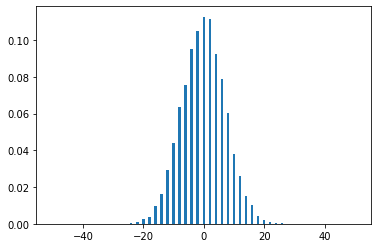
\includegraphics[scale=0.5]{figures/classical_distribution.png}
	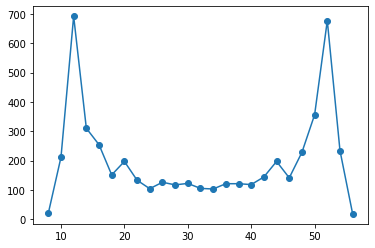
\includegraphics[scale=0.5]{figures/quantum_distribution.png}
	% To make sure citation doesn't appear in list of figures
	\caption [
	مقایسه‌ی توزیع احتمالی گشت گرافی کلاسیک و کوانتوم
	]{
	مقایسه‌ی توزیع احتمالی گشت گرافی کلاسیک (راست) و کوانتومی (چپ)
	\cite{cirq_qwalk}
	}
	\label{fig:walk_distr}
\end{figure}

\myequations{انحراف معیار گشت‌های کوانتوم و کلاسیک}
به طور خلاصه، الگوریتم گشت گراف کوانتومی، وضعیت گردش‌گر را در چند کیوبیت کدگذاری می‌کند و با فرض شروع مسیر گردش‌گر از یک ند خاص در گراف؛ در هر مرحله، با استفاده از یک کیوبیت سکه
\fnote{Coin qubit}
که در هر مرحله تحت تاثیر یک گیت هادامارد قرار می‌گیرد، وضعیت کیوبیت‌ها را به برهم‌نهی‌ای از وضعیت ندهای مجاور آن گراف می‌برد. نکته‌ای که باعث تفاوت حرکات گردش‌گر کلاسیک و کوانتومی می‌شود، اثر تداخل کوانتومی
\fnote{Quantum interference}
است که احتمالات حضور گردش‌گر در برخی نت‌ها را تقویت و در برخی دیگر، تضعیف می‌کند.
مقایسه‌ی توزیع احتمال مکان نهایی گردش‌گر در اجرای الگوریتم گشت بر روی گراف حلقوی‌ای با ۶ ند در حالت کلاسیک و در حالت کوانتومی‌ای که کیوبیت سکه‌ی آن در زمان
$t=0$
از وضعیت اولیه‌ی زیر شروع شده:
\begin{equation}
    |i\rangle = \frac{|0\rangle + i|1\rangle}{\sqrt{2}}
\end{equation}
\myequations{وضعیت اولیه‌ی کیوبیت‌ها در یک گشت کوانتومی}
در شکل
\ref{fig:walk_distr}
آمده است.
بیان ریاضی عمل‌گرهای الگوریتم گشت کوانتومی به صورت زیر است:
\begin{equation}
\begin{gathered}
    |q_t\rangle = |state_t\rangle \otimes |coin_t\rangle \\[3pt]
    U = |0\rangle \langle 0| \otimes \sum_j |j + 1\rangle \langle j| + |1\rangle \langle 1| \otimes \sum_j |j - 1\rangle
    \langle j| \\[3pt]
    S = U(H \otimes \mathbb{I}) \\[3pt]
    |q_{t+1}\rangle = S|q_t \rangle
\end{gathered}
\end{equation}
\myequations{بیان ریاضی عمل‌گرهای الگوریتم گشت کوانتومی}

که منظور از بردارهایی به شکل
$|j\rangle$
و 
$|j+1\rangle$
نمایش وضعیت کیوبیت‌های بردارهای وضعیت به شکل عدد طبیعی است که عمل‌گرهای جمع و تفریق حلقوی به آن‌ها اعمال می‌شود؛ به عنوان مثال:
\begin{equation}
    \begin{gathered}
        |7\rangle = |111\rangle \\[3pt]
        |7 + 1\rangle = |8 \hso mod \hso 8\rangle = |0\rangle = |000\rangle \\[3pt]
        |0 - 1\rangle = |-1 \hso mod \hso 8\rangle = |7\rangle = |111\rangle
    \end{gathered}
\end{equation}
\myequations{مثال عمل‌گرهای جمع و تفریق حلقوی در الگوریتم گشت کوانتومی}

الگوریتم پیشنهاد شده در 
\cite{miranda}
نمونه‌گیری از یک الگوریتم گشت کوانتومی روی یک گراف با ۸ ند است که تنها به ۳ کیوبیت نیاز دارد. این الگوریتم پس از اندازه‌گیری وضعیت گردش‌گر گراف در انتهای چند مرحله گشت، وضعیت
$|000\rangle$
را به عنوان سکوت، و ۷ وضعیت پایه‌ی دیگر را به عنوان ۷ نت ماژور (معادل کلیدهای سفید پیانو) در نظر می‌گیرد و بر اساس چندین بار اجرای این الگوریتم، قطعه‌ای در یک کلید ماژور تولید می‌کند.
\chapter{پیاده‌سازی و نتایج نو}

در این پروژه، (تا جایی که نویسنده اطلاع دارد) برای اولین بار از الگوریتم‌های یادگیری ماشین کوانتومی برای تولید موسیقی استفاده شده و همان‌طور که در بخش
\ref{sec:parts}
اشاره شد، شامل سه ماژول 
\lr{Midi, QLSTM} 
و
\lr{QuGAN}
است که در این فصل توضیحات کامل عملکرد آن‌ها شرح داده می‌شود.
شایان ذکر است که موسیقی‌های تولید شده توسط این مدل، دارای تندای
\fnote{Tempo}
ثابت هستند، به این معنا که فاصله‌ی بین نت‌های مختلف همیشه یکسان و برابر با ۵۰ میلی‌ثانیه است.
مدارهای کوانتومی این پروژه، با استفاده از کتاب‌خانه‌ی 
\lr{PennyLane}
که کتاب‌خانه‌ای مختص یادگیری ماشین کوانتومی است طراحی شده‌اند و بهینه‌سازی پارامترهای این مدارها، با استفاده از رابط کاربری بین این کتاب‌خانه و کتاب‌خانه‌ی
\lr{PyTorch}
انجام شده‌است.

\section{ماژول 
\lr{Midi}
} \label{sec:midi_module}
ماژول
\lr{Midi}
مسئولیت پیش‌پردازش داده‌ها برای استفاده از مدل‌های یادگیری ماشین کوانتومی را بر عهده دارد.
مجموعه داده‌ی این پروژه، شامل ۹۲ قطعه‌ی موسیقی پیانو به صورت فایل‌های 
\lr{midi}
است، هرکدام از این فایل‌ها، مجموعه‌ای از نت‌ها، آکوردها و زمان پخش آن نت/آکورد از ابتدای قطعه به میلی‌ثانیه است.
این ماژول، با استفاده از کتاب‌خانه‌ی 
\lr{Music21}
تنها یک‌بار پوشه‌ی شامل مجموعه داده‌ها را به صورت کامل بررسی کرده، نت‌های تمامی قطعات را به صورت متوالی در یک لیست ذخیره کرده و در نهایت در یک فایل واحد با نام
\lr{notes.pk}
ذخیره می‌کند. شایان ذکر است که در صورت برخورد با یک آکورد، نت‌های آن را استخراج کرده و همانند چند نت عادی که پشت سر هم پخش می‌شوند، آن‌ها را به لیست نت‌ها اضافه می‌کند.
در عین حال، برای قابل‌فهم کردن نت‌ها برای یک مدل یادگیری ماشین، یک نگاشت ۱-به-۱
از نت‌ها به اعداد طبیعی ساخته می‌شود.
این ماژول سپس در هر بار اجرای کد، با گرفتن پارامتری به نام
\lr{SequenceLength}
تعداد زیادی جفت ورودی و خروجی برای مدل یادگیری ماشین کوانتومی فراهم می‌کند؛ به این صورت:

\begin{equation}
    \begin{gathered}
    input_i = [inotes_{(i)}, ..., inotes_{(SequenceLength + i)}] \\[3pt]
    norm_i = \sqrt{\sum^{SequenceLength+i}_{k=i} (inotes_{(k)})^2 } \\[3pt]
    output_i = [inotes_{(SequenceLength + i + 1)}] \\[3pt]
    where \hso 0 \leq i \leq n - SequenceLength - 1 \hso ; \hso n = \#notes
    \end{gathered}
\end{equation}
\myequations{نحوه تولید ورودی و خروجی ماژول \lr{Midi}}
که در معادله‌ی بالا،
$inotes_{(i)}$
برابر با عدد طبیعی‌ای‌ست که معادل
$i$-
امین نت در مجموعه نت‌هاست.


\section{ماژول
\lr{QLSTM}
} \label{sec:qlstm_module}
هدف این ماژول، تولید موسیقی با استفاده از حافظه‌های طولانی کوتاه مدت کوانتومی است. در این بخش، جزئیات پیاده‌سازی این ماژول شرح داده می‌شوند.
در کتابخانه‌ی 
\lr{PyTorch}،
هر مدل آموزش‌پذیر یادگیری ماشین، زیرکلاسی از کلاس 
\lr{torch.nn.Module}
است. به همین دلیل، کلاس‌های این ماژول، همگی زیرکلاسی از
\lr{torch.nn.Module}
هستند.
یکی از توابع مهم کلاس
\lr{torch.nn.Module}،
تابع
\lr{forward}
است که در هر بار اجرا، مقداری داده به عنوان ورودی گرفته و با اعمال یک الگوریتم یادگیری ماشین به این ورودی‌ها، نتایج تولید شده توسط این الگوریتم را به عنوان خروجی می‌دهد.
این کلاس‌ها در زیر شرح داده می‌شوند.

\subsection{طراحی اولیه}
طراحی اولیه‌ی این ماژول، الهام گرفته از پیاده‌سازی‌های معمول تولید موسیقی با استفاده از حافظه‌های طولانی کوتاه مدت کلاسیک بود که در بخش زیر به این پیاده‌سازی‌های کلاسیک پرداخته می‌شود:
\subsubsection{پیاده‌سازی کلاسیک}
ایده‌ی کلی این پیاده‌سازی‌ها به این صورت است که در اولین مرحله،
$output_i$
های تولید شده در ماژول 
\lr{Midi}،
با استفاده از کدگذاری یک بارز\fnote{One-hot encoding} شکل جدیدی پیدا می‌کنند. این کدگذاری به این صورت انجام می‌شود که اگر 
\lr{n}
تعداد
$output_i$
وجود داشته باشد، داده‌ی
\lr{k}
ام این مجموعه که
$output_k$
نام دارد، تبدیل به برداری
\lr{n}
بعدی می‌شود که همه‌ی ورودی‌های آن صفر است و تنها 
\lr{k}
امین ورودی آن برابر با یک قرار می‌گیرد.
در این مساله، عدد 
\lr{n}
برابر با تعداد نت‌های منحصر به فرد موجود در لیست
\lr{notes}
تولید شده در ماژول
\lr{Midi}
در نظر گرفته می‌شود.
سپس، با گرفتن ابعاد بردارهای ورودی و خروجی گیت‌های بازگشتی به عنوان ورودی، ابعاد ماتریس‌های
\lr{W} و \lr{U}
که در معادله‌ی
\ref{eqn:lstm_gate}
تعریف شده بودند تعیین می‌شود و واحدهای بازگشتی با استفاده از این ابعاد و پارامتر حذفی که برابر با ۳.۰ است ساخته می‌شوند. پس از قرار دادن تعدادی لایه‌ی بازگشتی پشت سر هم، ابتدا خروجی‌های لایه‌های مختلف تحت تاثیر یک لایه‌ی خطی که در کتابخانه‌ی
\lr{PyTorch}
به صورت کلاس
\lr{torch.nn.Linear}
پیاده‌سازی شده است قرار می‌گیرند. کارکرد این لایه به این صورت است که با گرفتن سه عدد
$n, m$ و $b$
برداری 
$n$
بعدی را با استفاده از تبدیل خطی زیر، تبدیل به برداری
$m$
بعدی می‌کند:
% \vspace{-1mm}
\begin{equation}
\begin{gathered}
       y = Ax + b \\
       dim(A) = m * n
\end{gathered}
\end{equation}
\myequations{نحوه‌ی کارکرد کلاس \lr{torch.nn.Linear}}
% \vspace{-3mm}
دلیل وجود این لایه‌ی خطی این است که بردارهایی که توسط خروجی‌های واحدهای بازگشتی ساخته شده، تبدیل به بردارهایی با طول
\lr{n}
شوند.  این کار باعث می‌شود خروجی‌های مدل، با خروجی‌هایی که تحت کدگذاری یک بارز قرار گرفته بودند، قابل مقایسه شوند.
در انتها، بردار نهایی تولید شده به عنوان برداری از احتمالات خروجی داده شدن هر کدام از نت‌های موجود در لیست 
\lr{notes}
تعبیر می‌شود و تابع آنتروپی متقاطع
\fnote{Cross Entropy}
به عنوان تابع هزینه‌ی این مدل در نظر گرفته می‌شود.
تابع آنتروپی متقاطع به این صورت تعریف می‌شود که اگر
\lr{N}
عدد دسته‌بندی وجود داشته باشد و برداری 
\lr{N}
بعدی به نام 
\lr{x}
به عنوان ورودی به این تابع داده شود، خروجی آن به صورت معادله‌ی زیر خواهد بود:

\begin{equation}
    \begin{gathered}
       loss(x, class) = -log\big(\frac{exp(x[class])}{\sum_j exp(x[j])}\big) = -x[class] + log\big(\sum_j exp(x[j])\big) \\
       loss = \frac{
        \sum_{i=1}^{N} loss(i, class[i])
       }{N}
    \end{gathered}
\end{equation}
\myequations{تابع آنتروپی متقاطع}

در مراحل اولیه‌ی پروژه، این پیاده‌سازی کلاسیک به کمک کتابخانه‌ی
\lr{PyTorch}
به طور کامل انجام شد تا از انجام‌پذیر بودن کلیت مساله اطمینان حاصل شود.

\subsubsection{پیاده‌سازی کوانتومی}
در مرحله‌ی بعد، سعی شد تا با جایگزین کردن حافظه‌ی طولانی کوتاه مدت کلاسیک با یک حافظه‌ی طولانی کوتاه مدت کوانتومی، الگوریتمی کوانتومی برای تولید موسیقی طراحی شود. حافظه‌ی طولانی کوتاه مدت  کوانتومی استفاده شده در این بخش، بر اساس مدلی که در بخش
\ref{sec:qlstm}
معرفی شد طراحی شده است.
بعد از پیاده‌سازی و انجام تست‌های مختلف بر روی این پیاده‌سازی با استفاده از ابرپارامترهای متفاوت، به این نتیجه رسیده شد که این‌گونه پیاده‌سازی، تنها می‌تواند با یادگیری بر روی هر مجموعه داده، یک نت ثابت تولید کند. این مساله به این دلیل است که اختلاف بسیار زیادی بین تعداد نت‌های منحصر به فرد موجود در مجموعه داده و تعداد کیوبیت‌های قابل شبیه‌سازی بر روی کامپیوترهای کلاسیک وجود دارد؛ این امر باعث می‌شود که پارامترهای موجود در لایه‌ی
\lr{torch.nn.Linear}
مدل، نتوانند به تبدیل مناسبی از برداری با بعد پایین که از خروجی اندازه‌گیری‌های کیوبیت‌ها تولید شده است به برداری با بعدی به اندازه‌ی تعداد نت‌های منحصر به فرد موجود در مجموعه داده دست پیدا کنند. به همین خاطر، در نسخه‌ی کنونی پروژه معماری متفاوتی برای استفاده از حافظه‌های طولانی کوتاه مدت کوانتومی پیشنهاد شده که جزئیات آن به صورت کامل در بخش‌های بعدی بیان شده است.

% بخش کوانتومی ماژول
% \lr{QLSTM}
% بر اساس حافظه‌های طولانی کوتاه-مدت کوانتومی که در بخش
% \ref{sec:qlstm}
% معرفی شدند طراحی شده است.
% \newparagraph

\begin{figure}
    \centering
    \begin{quantikz}
            \lstick[wires=3]{$\ket{0}^{\otimes n\_qubits}$} & \gate[wires=3][2cm]{AE(x)} & \gate[wires=3][2cm]{RL_1(\theta_1)} &\qw &\ldots &\ & \gate[wires=3][2cm]{RL_k(\theta)} & \qw & \meter{}  \\
            & \qw & \qw & \qw & \ldots & & \qw & \qw & \meter{} \\
            & \qw & \qw & \qw & \ldots & & \qw & \qw & \meter{}
    \end{quantikz}
    \caption{نمایش دیداری مدار کوانتومی استفاده شده در حافظه‌ی طولانی کوتاه مدت کوانتومی}
    \label{fig:qrecursive}
\end{figure}

\newpage
\subsection{
کلاس
\lr{QLSTMCell}
}

\begin{algorithm}[t]
\caption{نحوه‌ی کارکرد یک واحد بازگشتی در حافظه‌ی طولانی کوتاه مدت کوانتومی} \label{alg:qlstmcell}
\lr{
    \begin{algorithmic}
        \STATE $c_{t-1}$ \hso $\leftarrow$ Cell state vector from the previous cell
        \STATE $h_{t-1}$ \hso $\leftarrow$ Hidden state vector from the previous cell
        \STATE $x_{t}$ \hso $\leftarrow$ Current cell's input
        \STATE drop \hso $\leftarrow$ Current cell's dropout value
        \STATE VQC\_forget \hso $\leftarrow$ pre-generated quantum recurrent gate
        \STATE VQC\_input \hso $\leftarrow$ pre-generated quantum recurrent gate
        \STATE VQC\_update \hso $\leftarrow$ pre-generated quantum recurrent gate
        \STATE VQC\_output \hso $\leftarrow$ pre-generated quantum recurrent gate
        \STATE $y_{t} = [h_{t-1} \hso ; \hso x]$
        \STATE $f_{t} = sigmoid(VQC\_forget(y_{t}))$
        \STATE $i_{t} = sigmoid(VQC\_input(y_{t}))$
        \STATE $g_{t} = sigmoid(VQC\_update(y_{t}))$
        \STATE $o_{t} = sigmoid(VQC\_output(y_{t}))$
        \STATE $c_{t} = (f_{t} * c_{t}) + (i_{t} * g_{t})$
        \STATE $h_{t} = o_{t} * tanh(c_{t})$
        \STATE $h_{t} = dropout(h_{t}, drop)$
    \end{algorithmic} 
}
\end{algorithm}
\myalgorithms{
   نحوه‌ی کارکرد یک واحد بازگشتی در حافظه‌ی طولانی کوتاه مدت کوانتومی
}

هر واحد بازگشتی کوانتومی این الگوریتم در کلاس
\lr{QLSTMCell}
تعریف شده.
ورودی‌های مهمی که برای ساختن نمونه‌ای از این کلاس لازم است به شرح زیر هستند:
\begin{itemize}
    \item 
    \lr{n\_qubits}
    تعداد کیوبیت‌های استفاده شده در مدارهای کوانتومی این واحد بازگشتی است.
    \item
    \lr{n\_qlayers}
    تعداد لایه‌های موجود در قسمت پارامتردار مدارهای کوانتومی را تعیین می‌کند.
    \item
    \lr{hidden\_size}
    ابعاد داده‌های ورودی و خروجی واحد بازگشتی را تعیین می‌کند.
\end{itemize}

این کلاس سپس با استفاده از پارامترهای دریافت شده، چهار مدار کوانتومی برای گیت‌های بازگشتی می‌سازد.
هر کدام از این مدارهای کوانتومی، از ترکیب تابع کدگذاری
\lr{AmplitudeEmbedding}
و تابع پارامتریک
\lr{RandomLayers}
کتابخانه‌ی
\lr{PennyLane}
ساخته شده است.

هر تابع
\lr{AmplitudeEmbedding}
با دریافت ورودی‌ای با ابعاد
$2^n$،
آن را در 
$n$
کیوبیت هدف به صورت زیر کدگذاری می‌کند:
\begin{equation} \label{eqn:midi_data}
    \begin{gathered}
       input = [x_0, x_1, \dots, x_{2^n-1}] \hst ; \hst x_i \in \mathbb{R} \\[3pt]
       norm = \sqrt{\sum^{2^n}_{i=0} x_i^2 } \\[3pt]
       output = \frac{x_0}{norm} |00...0\rangle + \frac{x_1}{norm} |00...1\rangle + ... + \frac{x_{2^n-1}}{norm} |11...1\rangle
    \end{gathered}
\end{equation}
\myequations{
نحوه‌ی کارکرد تابع
\lr{AmplitudeEmbedding}
}

و هر تابع 
\lr{RandomLayers}
با دریافت یک ورودی با ابعاد
$(L, k)$
و یک عدد طبیعی
\lr{seed}
،تعداد
$L$
لایه‌ی پارامتریک را با استفاده از
\lr{seed}
به صورت تصادفی تولید می‌کند.
هر لایه‌ی تولید شده توسط
\lr{RandomLayers}
شامل ترکیبی از 
$k$
گیت کوانتومی پارامتریک و تعدادی گیت 
$CNOT$
است.


نمایش دیداری این گیت‌های بازگشتی کوانتومی، در شکل
\ref{fig:qrecursive}
آمده است که این شکل، دقیقا حالت خاصی از شکل
\ref{fig:qml_visualization}
است که در آن، از 
\lr{AmplitudeEmbedding}
برای لایه‌ی کدگذاری و از
\lr{RandomLayers}
برای لایه‌ی پارامتریک استفاده شده است.
لازم به ذکر است که در این شکل به جهت اختصار از عبارت
\lr{AE}
به جای
\lr{AmplitudeEmbedding}
و از عبارت
\lr{RL}
به جای 
\lr{RandomLayers}
استفاده شده است.

پس هر واحد بازگشتی در پیاده‌سازی فعلی، یک
\lr{QLSTMCell}
است که مدارهای کوانتومی آن، از پشت سر هم قرار گرفتن زیرمدارهای تولید شده توسط
\lr{AmplitudeEmbedding}
و
\lr{RandomLayers}
ساخته شده‌اند و در نهایت، آرایه‌ای متشکل از امیدریاضی اندازه‌گیری جداگانه‌ی تک‌تک کیوبیت‌های هر مدار به عنوان خروجی آن مدار در نظر گرفته می‌شود.
فرم شبه‌کدی الگوریتم اجرا شده در هر بار اجرای تابع
\lr{forward}
یک کلاس
\lr{QLSTMCell}
به صورت کامل در الگوریتم
\ref{alg:qlstmcell}
آمده است. در این الگوریتم، متغیرهای
$c_{t-1}$ و
$h_{t-1}$
که به ترتیب بردار وضعیت واحد و بردار وضعیت پنهان واحد بازگشتی قبلی هستند به صورت ورودی داده می‌شوند. متغیر
$x_{t}$
نیز که ورودی واحد بازگشتی کنونی است، از مجموعه داده‌ی پروژه به صورت ورودی به این الگوریتم داده می‌شود. هم‌چنین، توابع
\lr{VQC\_forget}،
\lr{VQC\_input}،
\lr{VQC\_update} و
\lr{VQC\_output}
مدارهای کوانتومی‌ای هستند که از پیش با استفاده از پارامترهای
\lr{n\_qubits}
و
\lr{n\_qlayers}
ساخته شده‌اند و ساختارشان به صورتی که در شکل
\ref{fig:qrecursive}
ترسیم شده قرار دارد.
\lr{drop}
که پارامتر حذف این واحد بازگشتی است نیز به عنوان ورودی به این الگوریتم داده می‌شود.

\begin{algorithm}[t]
\caption{نحوه‌ی کارکرد یک حافظه‌ی طولانی کوتاه مدت کوانتومی} \label{alg:full_qlstm}
\lr{
    \begin{algorithmic}
        \STATE n\_layers \hso $\leftarrow$ Number of QLSTMCell's present in this QLSTM
        \STATE QLSTMCells \hso $\leftarrow$ A list of initialized QLSTMCell's
        \STATE inputs \hso $\leftarrow$ A list of inputs generated by the Midi module
        \STATE outputs \hso $\leftarrow$ Empty list
        \STATE $h_{t} = [0, \dots, 0]$
        \STATE $c_{t} = [0, \dots, 0]$
        \FOR {$ i=0 \to$ n\_layers}
            \STATE $h_{t}, c_{t} = QLSTMCells[i](inputs[i], h_{t}, c_{t})$
            \STATE outputs.add$(c_{t})$
        \ENDFOR
    \end{algorithmic} 
}
\end{algorithm}
\myalgorithms{
   نحوه‌ی کارکرد یک حافظه‌ی طولانی کوتاه مدت کوانتومی
}

\subsection{
کلاس
\lr{QLSTM}
}

این کلاس با دریافت ورودی‌ای با نام
\lr{n\_layers}،
تعداد
\lr{n\_layers}
لایه از 
\lr{QLSTMCell}
ها را در کنار هم قرار می‌دهد و تغییرات لازم برای رد کردن خروجی‌های هرکدام از این لایه‌ها به عنوان ورودی لایه‌ی بعدی را انجام می‌دهد. این کلاس در هر بار اجرا، آرایه‌ای به نام
\lr{outputs}
که مجموعه‌ی خروجی‌های تولید شده توسط 
\lr{n}
لایه از واحدهای بازگشتی کوانتومی است را خروجی می‌دهد.
فرم شبه‌کدی الگوریتم اجرا شده در هر بار اجرای تابع
\lr{forward}
کلاس 
\lr{QLSTM}
به صورت کامل در الگوریتم
\ref{alg:full_qlstm}
آمده است.

\subsection{
کلاس
\lr{QLSTMusic}
}
این کلاس با گرفتن ورودی و خروجی‌های تولید شده از ماژول
\lr{Midi}
و یک عدد طبیعی به نام
\lr{n\_epochs}،
به تعداد
\lr{n\_epochs}
بار
ورودی و خروجی‌ها را به یک 
\lr{QLSTM}
رد می‌کند و بعد از انجام پس‌پردازش روی خروجی‌های تولید شده، پارامترهای آن را برای کمینه‌کردن یک تابع هزینه بهینه‌سازی می‌کند. چگونگی انجام این پس‌پردازش به طور کامل در بخش بعد شرح داده شده است.

\subsection{پس‌پردازش} \label{sec:qlstm_post}
\begin{algorithm}[t]
\caption{پس‌پردازش ماژول \lr{QLSTM}}  \label{alg:qlstmpost}
\lr{
    \begin{algorithmic}
        \STATE $raw\_model\_output_i = QLSTMCells[i](input_i)$
        \STATE $model\_output_i = mean(raw\_model\_output_i)$
        \STATE $model\_output_i = model\_output_i * norm_i$
    \end{algorithmic}
}
\end{algorithm}
\myalgorithms{
    پس‌پردازش ماژول
    \lr{QLSTM}
}
هر لایه از
\lr{QLSTM}
که شامل
$n$
کیوبیت باشد، 
$n$
خروجی که هر کدام از آن‌ها عددی در بازه‌ی
$[-1, 1]$
است تولید می‌کند. به همین دلیل، برای تبدیل کردن این اعداد به اعداد طبیعی‌ای که معادل نت‌های مجموعه داده باشند، باید روی خروجی‌ها پس‌پردازش انجام داد.
پس‌پردازش پیشنهادی در این مرحله، در الگوریتم
\ref{alg:qlstmpost}
آمده است. در این الگوریتم، متغیرهای
$input_i$
و
$norm_i$
طبق معادله‌ی
\ref{eqn:midi_data}
تعریف شده‌اند،
$raw\_model\_output_i$
خروجی اولیه‌ای است که از مدار کوانتومی گرفته می‌شود و
$model\_output_i$
خروجی نهایی بعد از پس‌پردازش است.



% برای هر
% \lr{QLSTMCell}،
% پس از پاس‌داده‌شدن
% $input_i$
% به شکلی که در معادله‌ی
% \ref{eqn:midi_data}
% تعریف شده، 
% یک
% $modelOutput_i$
% تولید می‌شود که شامل
% $n$
% عدد است.
% ابتدا از خروجی‌های داده‌شده توسط هر کدام از واحدهای بازگشتی میانگین گرفته می‌شود و سپس با ضرب این میانگین
% در
% $norm_i$،
% عدد طبیعی معادل نت پیشنهادی هر
% \lr{QLSTMCell}
% تولید می‌شود.

\subsection{تابع هزینه}
به علت این‌که ممکن است عدد طبیعی معادل نت پیشنهادی، بزرگ‌تر یا کوچک‌تر از عدد طبیعی معادل نت خروجی مجموعه داده باشد، از تابع خطای میانگین مربعات که در معادله‌ی
\ref{eqn:mse}
معرفی شد، به عنوان تابع هزینه استفاده می‌شود.
علت مناسب بودن این تابع هزینه، این است که در هنگام ساخت نگاشت یک به یک از نت‌ها به اعداد طبیعی، مرتب‌سازی به گونه‌ای انجام شد که هرچه‌قدر فرکانس نت‌ها به هم نزدیک‌تر باشد، اعداد طبیعی متناظر آن‌ها نیز به هم نزدیک‌تر باشند.

در نهایت، تابع
\lr{generate\_notes}
با گرفتن پارامتر
\lr{n\_notes}
با چندین‌بار اجرای الگوریتم‌های یادگیری ماشین و پس‌پردازش، به تعداد
\lr{n\_notes}
نت موسیقی جدید تولید کرده و با قرار دادن فاصله‌هایی به اندازه‌ی پنجاه میلی‌ثانیه بین آن‌ها، نتایج حاصل را در یک فایل با پسوند
\lr{midi}
ذخیره می‌کند.


\section{
ماژول
\lr{QuGAN}
}
ماژول
\lr{QuGAN}
بر اساس شبکه‌های زایای دشمن‌گونه‌ی کوانتومی که در بخش
\ref{sec:qugan}
معرفی شد طراحی شده است.
این ماژول نیز همانند ماژول
\lr{QLSTM}
از ماژول
\lr{Midi}
برای پیش‌پردازش داده‌ها استفاده می‌کند.

این ماژول به طور کلی شامل سه زیرمدار کوانتومی است. از ترکیب‌های مختلف این سه زیرمدار، سه مدار کوانتومی تشکیل می‌شود که توضیح کارکرد آن‌ها در زیر آمده است:

\begin{itemize}
    \item زیرمدار اول که در کد پروژه توسط تابع
    \lr{encode\_music}
    ساخته می‌شود، با دریافت نت‌هایی به عنوان ورودی، آن‌ها را با استفاده از تابع
    \lr{AmplitudeEmbedding}
    در کیوبیت‌های سیستم کدگذاری می‌کند.
    
    \item زیرمدار دوم که زیرمداری پارامتریک است و در کد پروژه توسط تابع
    \lr{discriminator}
    ساخته می‌شود، با استفاده از تابع
    \lr{RandomLayers}
    لایه‌هایی پارامتریک تولید می‌کند. این لایه‌ها سعی در تشخیص واقعی یا ساختگی بودن داده‌های موجود در کیوبیت‌ها دارند و عمل‌کرد متمایزکنندگی شبکه را پیاده‌سازی می‌کنند.
    خروجی این زیرمدار، آرایه‌ای متشکل از امیدریاضی اندازه‌گیری تک‌تک کیوبیت‌های سیستم به صورت مجزا است.
    
    \item زیرمدار سوم، همانند زیر مدار دوم مداری پارامتریک است، اما سعی در تولید داده‌هایی ساختگی از روی کیوبیت‌هایی که مقداری نویز به عنوان داده‌ی اولیه بر روی آن‌ها کدگذاری شده‌اند دارد. این زیرمدار در کد پروژه توسط تابع
    \lr{music\_generator}
    ساخته می‌شود و عملکرد زایایی شبکه را پیاده‌سازی می‌کند.
\end{itemize}

و مدارهای کوانتومی این ماژول، به این شکل ساخته شده‌اند:
\begin{itemize}
    \item
    مدار اول که
    \lr{real\_music\_discriminator}
    نام دارد،
    ابتدا به کمک تابع
    \lr{encode\_music}
    تعدادی نت از مجموعه داده گرفته و آن‌ها را در کیوبیت‌های سیستم کدگذاری می‌کند، سپس زیرمدار
    \lr{discriminator}
    سعی می‌کند با بهینه‌سازی پارامترهای خود تشخیص دهد آیا داده‌ها واقعی هستند یا خیر.
    
    \item
    مدار دوم که
    \lr{generated\_music\_discriminator}،
    نام دارد، ابتدا با گرفتن مقداری نویز به عنوان ورودی، آن نویزها را توسط
    \lr{encode\_music}
    در سیستم کدگذاری می‌کند، سپس زیرمدار \\
    \lr{music\_generator}
    با بهینه‌سازی پارامترهای خود، اقدام به ساخت داده‌ی جدیدی از روی نویز کدگذاری شده می‌کند و در نهایت، زیرمدار
    \lr{discriminator}
    سعی می‌کند با بهینه‌سازی پارامترهای خود، تشخیص دهد آیا داده یکی از داده‌های واقعی است یا خیر.
    
    \item
    مدار سوم که
    \lr{final\_music\_generator}
    نام دارد، با ترکیب زیرمدار‌های
    \lr{encode\_music}
    و \\
    \lr{music\_generator}
    ابتدا مقداری نویز را در سیستم کدگذاری کرده و سپس آرایه‌ای متشکل از امیدریاضی اندازه‌گیری تک‌تک کیوبیت‌های سیستم را به عنوان خروجی تولید می‌کند که نتیجه‌ی نهایی الگوریتم، از این خروجی ساخته می‌شود.
    
\end{itemize}
نکته‌ی اصلی این است که بعد از هربار اجرای مدارهای اول و دوم، وزن‌های زیرمدار
\lr{discriminator}
آن‌ها با هم همگام می‌شوند، چراکه در کل برنامه باید تنها یک
\lr{discriminator}
وجود داشته‌باشد.

بعد از ساخته‌شدن این مدارها، با استفاده از توابع هزینه‌ی معرفی شده در معادله‌ی
\ref{eqn:qugan_cost}
پارامترهای زیرمدارهای 
\lr{discriminator}
و
\lr{music\_generator}
بهینه‌سازی می‌شوند؛ سپس پارامترهای زیرمدار
\lr{music\_generator} 
موجود در مدار دوم با پارامترهای مدار سوم همگام‌سازی شده و پس از پس‌پردازش خروجی‌های مدار سوم، موسیقی تولید می‌شود.

\subsection{پس‌پردازش}

\begin{algorithm}[t]
\caption{پس‌پردازش ماژول \lr{QuGAN}} \label{alg:quganpost}
\lr{
    \begin{algorithmic}
        \STATE $model\_output_i = model(input_i)$
        \STATE $model\_output_i = (model\_output_i + 1) * norm_i$
        \STATE $counter = 1$
        \WHILE {$model\_output_i \not\in mapping.keys()$}
        \STATE $model\_output_i = model\_output_i * counter / (counter+1)$
        \STATE $model\_output_i = model\_output_i.to\_int()$
        \STATE $counter = counter + 1$
        \ENDWHILE
    \end{algorithmic} 
}
\end{algorithm}
\myalgorithms{
    الگوریتم پس‌پردازش ماژول
    \lr{QuGAN}
}

به همان دلیل ارائه شده در بخش
\ref{sec:qlstm_post}،
داده‌های این ماژول نیز نیاز به پس‌پردازش دارد، اما این ماژول برای تولید قطعات موسیقی آهنگین‌تر، نیاز به پس‌پردازش متفاوتی دارد.
پس‌پردازش استفاده شده در این ماژول طبق الگوریتم
\ref{alg:quganpost}
عمل می‌کند.
در این الگوریتم، همانند پس‌پردازش ماژول
\lr{QLSTM}،
متغیرهای
$input_i$
و
$norm_i$
طبق معادله‌ی
\ref{eqn:midi_data}
تعریف شده‌اند. 
منظور از 
\lr{mapping}
همان نگاشت یک به یک از نت‌ها به اعداد طبیعی است و
$model\_output_i$
خروجی نهایی بعد از پس‌پردازش،
است.
در نهایت، تابع
\lr{generate\_notes}
با گرفتن پارامتر
\lr{n\_notes}
با چندین‌بار اجرای الگوریتم، به تعداد
\lr{n\_notes}
نت موسیقی جدید تولید کرده و آن‌ها را در یک فایل با پسوند
\lr{midi}
ذخیره می‌کند.

\chapter{نتیجه‌گیری}

در این پروژه‌ی کارشناسی، سعی شد تا به بررسی محاسبات کوانتومی، یادگیری ماشین، تئوری موسیقی و تلاقی این سه حوزه برای تولید موسیقی‌های بدیع پرداخته شود. به نظر می‌رسد که تا به حال تلاش‌های کمی در راستای بررسی این تلاقی صورت گرفته است. با این وجود که به خاطر خواص موجی فیزیک کوانتومی و خواص موجی نت‌های موسیقی، احتمال داده می‌شود که پتانسیل‌های بسیار زیادی در این زمینه وجود داشته باشد.
ماحصل این پروژه، برنامه‌ی نرم‌افزاری‌ای است که با استفاده از یک مجموعه‌داده و چندین کتاب‌خانه‌ی پرکاربرد، موسیقی‌های بدیعی تولید می‌کند.

یک نکته حائز اهمیت این است که یادگیری این الگوریتم‌ها به نسبت سریع است و لزوما به تعداد کیوبیت‌های زیاد یا مدارهای عمیق برای تولید قطعات موسیقی آهنگین احتیاجی ندارد.
نکته حائز اهمیت دیگر این است که الگوریتم‌های پیاده‌سازی شده در این کتاب‌خانه، محدود به همین مجموعه داده نیستند و می‌توان با تزریق مجموعه داده‌ی دیگری (به عنوان مثال، اصوات متعلق به سازهای دیگر، همچون گیتار و درام) به آن، نتایج متفاوتی دریافت کرد.

در نهایت، کد این پروژه و ۴ نمونه موسیقی تولید شده با استفاده از آن را می‌توان در مخزن گیت‌هاب
\lr{Maqneta}
\cite{Maqenta}
مشاهده کرد.

\section{کارهای آینده}
همان‌طور که اشاره شد، هنوز جنبه‌های بسیاری از این حوزه کشف‌نشده باقی مانده‌اند. به عنوان مثال، الگوریتم متفاوتی
\cite{bausch2020recurrent}
برای شبکه‌های عصبی بازگشتی کوانتومی نیز ارائه شده‌است که در این پروژه، امکان تولید موسیقی با استفاده از این الگوریتم بررسی نشده است. هم‌چنین، الگوریتم‌های کلاسیکی برای تولید موسیقی با استفاده از یادگیری تقویتی
\fnote{Reinforcement learning}
و یادگیری انتقالی
\fnote{Transfer learning}
نیز وجود دارند و با توجه به این‌که نسخه‌ای کوانتومی از هر دوی این الگوریتم‌ها موجود است
\cite{Mari_qtransfer}
\cite{Daoyi_QReinforce}
احتمالا بتوان با بررسی آن‌ها نیز به تولید موسیقی پرداخت.

در حال حاضر، فعالیت‌هایی در این حوزه در جریان است. به عنوان مثال، کنفرانس
\lr{ISQCMC}
\cite{ISQCMC}
که در اواخر ماه نوامبر سال میلادی جاری برگزار خواهد شد، به برخی جنبه‌های دیگر تولید موسیقی با استفاده از محاسبات کوانتومی، همانند
تولید موسیقی با استفاده از اتوماتاهای سلولی کوانتومی
\fnote{Quantum cellular automata}
خواهد پرداخت.

% \chapter{خروجی و آزمون‌ها}

در این فصل سعی شده است تا با ارائه تعدادی تصاویر از محیط سامانه و عملکرد آن، خروجی سامانه و همچنین برخی از آزمون‌های تولید شده نیز ارائه شود. البته تعداد بسیار بیشتری تصویر و بخش قابل ارائه بود اما در این‌صورت حجم این گزارش بسیار زیاد می‌شد. همچنین  بدلیل این‌که جزئیات کار سامانه در فصول قبلی شرح داده شده از توضیح تصاویر فوق صرف‌نظر شده است.

\section{سامانه اصلی}

\subsection{ساختار فایل‌ها}

\begin{figure}[H]
	\centering
	\includegraphics[scale=0.5]{files}
	\caption{فایل‌های سامانه اصلی}
	\label{fig:files}
\end{figure}

\subsection{خروجی سامانه اصلی}

\begin{figure}[H]
	\centering
	\includegraphics[scale=0.45]{backend}
	\caption{درخواست ازمایشی دریافت پیشنهاد مبتنی بر مکان}
	\label{fig:backend}
\end{figure}


\newpage

\subsection{خروجی نرم‌افزار کاربردی}

\begin{figure}[H]
	\centering
	\includegraphics[scale=0.1]{1}
	\includegraphics[scale=0.1]{2}
	\includegraphics[scale=0.1]{3}
	\caption{به ترتیب از راست، لیست صفحه اصلی، لیست محصولات یک فروشگاه، صفحه یک محصول}
	\label{fig:app1}
\end{figure}

\begin{figure}[H]
	\centering
	\includegraphics[scale=0.1]{4}
	\includegraphics[scale=0.1]{5}
	\includegraphics[scale=0.1]{6}
	\caption{به ترتیب از راست، صفحه افزودن فروشگاه، صفحه تغییر یک محصول، صفحه مشاهده و آمارگیری لیست کوپن‌ها}
	\label{fig:app2}
\end{figure}

\section{آزمون سامانه}

\begin{figure}[H]
	\centering
	\includegraphics[scale=0.3]{test1}
	\caption{آزمون واحد تابع خطی‌ساز اشیا}
	\label{fig:test1}
\end{figure}


\begin{figure}[H]
	\centering
	\includegraphics[scale=0.4]{test2}
	\caption{آزمون واحد تولید بلیت با \lr{JWT}}
	\label{fig:test2}
\end{figure}


\begin{figure}[H]
	\centering
	\includegraphics[scale=0.3]{test3}
	\caption{آزمون واحد توابع کمکی کار با آرایه \lr{ArrayFilter}}
	\label{fig:test3}
\end{figure}




% \chapter{پیشنهادات و جمع‌بندی}

\section{کارهای آینده}

از مهم‌ترین اقداماتی که برای بهبود این پروژه می‌توان انجام داد، حل چالش بوجود آمده در زمینه پرس‌وجوهای مکانی مونگو است. به این‌صورت که می‌توان روشی که فصل 5 پیشنهاد شد را پیاده‌سازی کرد و تاثیر آن را بر عملکرد سامانه اندازه گرفت. زیرا همان‌طور که توضیح داده شده بود، این چالش در عمل چندان مشکل‌ساز نخواهد بود، اما درصورتی‌که اصلاح آن با روش پیشنهاد شده تاثیر مخرب ناچیزی بر عملکرد سامانه داشته باشد، اصلاح و غلبه بر آن مفید خواهد بود.\\

علاوه بر این، همانطور که تاکید شد، وظیفه اصلی این پروژه ارائه پیشنهاداتی از محصولات فروشگاه‌ها به کاربرانی است که یا از نظر موقعیت مکانی، احتمال گذر آن‌ها از آن فروشگاه‌ها بالاست و یا از پیش، علاقه‌مندی آن‌ها به آن محصولات مشخص شده است. موارد دیگری نیز می‌توان بعنوان کارهای فراتر از این پروژه انجام داد؛ برای مثال،

\begin{enumerate}

	\item می‌توان با تحلیل موقعیت مکانی هر کاربر در طول روز، مکان‌هایی که احتمالا فروشگاه هستند، ولی در این سامانه هنوز ثبت نشده‌اند را بعنوان نقطه مورد علاقه  در سامانه ثبت کرد تا پس از بررسی پشتیبان سامانه، بعنوان فروشگاه اضافه شود.
	\item پس از توافق با شرکت‌های ارائه دهنده خدمات تاکسی اینترنتی، می‌توان برای مسافرین این تاکسی‌ها درطول مسیر، پیشنهاداتی را ارائه داد که در صورت توقف برای خرید از فروشگاه پیشنهاد شده، هزینه سفر آن‌ها بصورت رایگان و از طرف این سامانه پرداخت شود.
	\item علاوه بر پیشنهاد مبتنی بر موقعیت مکانی و محصولات مشابه موردعلاقه کاربر، می‌توان پیشنهادات را از زنجیره‌هایی از مشتریانی که به فروشگاه‌های مشابهی مراجعه کرده‌اند نیز بدست آورد. در اینصورت، این سامانه عملا از ویژگی‌های یک شبکه اجتماعی مبتنی بر مکان برخوردار خواهد شد.
	
\end{enumerate}

\newpage

\section{جمع‌بندی}

امروزه بسیاری از سامانه‌های تجاری، اقدام به ارائه پیشنهادات به کاربران خود مطابق با سلیقه آن‌ها می‌کنند. اگر خدمات ارائه شده حضوری باشند و در ارائه این پیشنهادات، موقعیت مکانی کاربران بعنوان یک شاخص مهم مورد توجه قرار گیرد، می‌تواند مشتریان قابل توجهی به خود جذب نماید. سامانه تولید شده در این پروژه شامل اجزای مختلفی از جمله زیرساخت سامانه، نرم‌افزار کاربردی تلفن همراه هوشمند و پنل تحت وب برای مدیران است که باید در تعامل با یکدیگر، اهداف اصلی تعیین شده برای این پروژه را محقق نمایند. خدمت ارائه شده از طریق این نرم‌افزار، نمایش اطلاعات محصولات و فروشگاه‌های متنوع به کاربران علاقه‌مند و ارائه کوپن‌های تخفیف به آن‌هاست. درفرآیند تولید این سکوی نرم‌افزاری، چالش‌های مختلفی اعم از چالش‌های فرآیندی (از جمله نحوه دسته‌بندی وظایف)،‌ الگوریتمی (مانند نحوه محاسبه علاقه‌مندی‌ها در پایگاه‌داده استفاده شده) و معماری (مانند نحوه انتقال داده‌های محلی در طول نرم‌افزار تلفن همراه هوشمند کاربر) وجود داشته که سعی شده تا حد امکان با راه‌حل‌های مناسبی رفع شده و مسیر توسعه این سامانه هموار شود. کار انجام شده‌ی پیشِ‌رو، نقطه پایانی برای این پروژه نبوده و می‌توان ایده‌های زیادی برای پیشرفت و مسیر آینده این پروژه متصوّر شد؛ از جمله مواردی که در بخش قبلی توضیح داده شد.\\

کدهای پیاده‌سازی شده این سامانه در سه منبع از سامانه کنترل نسخه گیت‌هاب در آدرس‌های زیر موجود است:

\begin{enumerate}
	\item کد سامانه اصلی: \url{https://github.com/mmkhmmkh/LBSR_backend}
	\item کد نرم‌افزار کاربردی تلفن‌های هوشمند: \url{https://github.com/mmkhmmkh/LBSR_rn}
	\item کد پنل مدیران: \url{https://github.com/mmkhmmkh/LBSR_admin}
\end{enumerate}



%--------------------------------------------------------------------------appendix( مراجع و پیوست ها)
\chapterfont{\vspace*{-2em}\centering\LARGE}%

\appendix
\bibliographystyle{plain-fa}
\bibliography{references}
%\chapter*{‌پیوست}
\markboth{پیوست}{}
\addcontentsline{toc}{chapter}{پیوست}
موضوعات مرتبط با متن گزارش پایان نامه كه در يكی از گروه‌های زير قرار می‌گيرد، در بخش پيوست‌ها آورده شوند:
\begin{enumerate}
\item  اثبات های رياضی يا عمليات رياضی طولانی‌.‌
\item داده و اطلاعات نمونه (های) مورد مطالعه (\lr{Case Study}) چنانچه طولانی باشد‌.‌
\item نتايج كارهای ديگران چنانچه نياز به تفصيل باشد‌.‌
\item مجموعه تعاريف متغيرها و پارامترها، چنانچه طولانی بوده و در متن به انجام نرسيده باشد‌.‌
\end{enumerate}
% براي شماره‌گذاري روابط، جداول و اشكال موجود در پيوست‌ از ساختار متفاوتي نسبت به متن اصلي استفاده مي‌شود كه در زير به‌عنوان نمونه نمايش داده شده‌است. 
% \begin{equation}
%F=ma
%\end{equation}
\section*{کد میپل }
\begin{latin}
\begin{verbatim}

with(DifferentialGeometry):
with(Tensor):
DGsetup([x, y, z], M)
																	frame name: M
a := evalDG(D_x)
																	D_x
b := evalDG(-2 y z D_x+2 x D_y/z^3-D_z/z^2)


\end{verbatim}
\end{latin}
%--------------------------------------------------------------------------dictionary(واژه نامه ها)
%اگر مایل به داشتن صفحه واژه‌نامه نیستید، خط زیر را غیر فعال کنید.
\parindent=0pt
%%
\chapter*{واژه‌نامه‌ی فارسی به انگلیسی}
\pagestyle{style9}

\addcontentsline{toc}{chapter}{واژه‌نامه‌ی فارسی به انگلیسی}
%%%%%%
\begin{multicols*}{2}

{\bf آ}
\vspace*{3mm}


\farsiTOenglish{اسکالر}{Scalar}


\vspace*{3mm}
{\bf ب}
\vspace*{3mm}

\farsiTOenglish{بالابر}{Lift}


\vspace*{3mm}
{\bf پ}
%%\vspace*{3mm}

\farsiTOenglish{پایا}{Invariant}



\vspace*{3mm}
{\bf ت}
%%\vspace*{3mm}

\farsiTOenglish{ تناظر }{Correspondence}


\vspace*{3mm}
{\bf ث}
%%\vspace*{3mm}

\farsiTOenglish{ثابت‌ساز}{Stabilizer}

\vspace*{3mm}
{\bf ج}
%%\vspace*{3mm}

\farsiTOenglish{جایگشت}{Permutation}



\vspace*{3mm}
{\bf چ}
%%\vspace*{3mm}


\farsiTOenglish{چند جمله‌ای }{Polynomial}

\vspace*{3mm}
{\bf ح}
%%\vspace*{3mm}

\farsiTOenglish{حاصل‌ضرب دکارتی}{Cartesian product}


\vspace*{3mm}
{\bf خ}
%%\vspace*{3mm}

\farsiTOenglish{خودریختی}{Automorphism}

\vspace*{3mm}
{\bf د}
%%\vspace*{3mm}

\farsiTOenglish{درجه}{Degree}


\vspace*{3mm}
{\bf ر}
%%\vspace*{3mm}


\farsiTOenglish{ریزپردازنده}{microprocessor}


\vspace*{3mm}
{\bf ز}
%%\vspace*{3mm}


\farsiTOenglish{زیرمدول}{Submodule}


\vspace*{3mm}
{\bf س}
%%\vspace*{3mm}

\farsiTOenglish{سرشت}{Character}


\vspace*{3mm}
{\bf ص}
%%\vspace*{3mm}

\farsiTOenglish{صادقانه}{Faithful}

\vspace*{3mm}
{\bf ض}
%%\vspace*{3mm}

\farsiTOenglish{ضرب داخلی}{Inner product}

\vspace*{3mm}
{\bf ط}
%%\vspace*{3mm}


\farsiTOenglish{طوقه}{Loop}


\vspace*{3mm}
{\bf ظ}
%%\vspace*{3mm}


\farsiTOenglish{ظرفیت}{Valency}
 
\vspace*{3mm}
{\bf ع}
%%\vspace*{3mm}


\farsiTOenglish{عدم مجاورت}{Nonadjacency}



\vspace*{3mm}
{\bf ف}
%%\vspace*{3mm}

\farsiTOenglish{فضای برداری}{Vector space}



\vspace*{3mm}
{\bf ک}
%%\vspace*{3mm}

\farsiTOenglish{کاملاً تحویل‌پذیر}{Complete reducibility}


\vspace*{3mm}
{\bf گ}
%%\vspace*{3mm}


\farsiTOenglish{گراف}{Graph}



\vspace*{3mm}
{\bf م}
%%\vspace*{3mm}

\farsiTOenglish{ماتریس جایگشتی}{Permutation matrix }


\vspace*{3mm}
{\bf ن}
%%\vspace*{3mm}

\farsiTOenglish{ناهمبند}{Disconnected}


\vspace*{3mm}
{\bf و}
%%\vspace*{3mm}

\farsiTOenglish{وارون‌پذیر}{Invertible}


\vspace*{3mm}
{\bf ه}
%%\vspace*{3mm}

\farsiTOenglish{همبند}{Connected}



\vspace*{3mm}
{\bf ی}
%%\vspace*{3mm}

\farsiTOenglish{یال}{Edge}




\end{multicols*}%
%%%%%%%
\chapter*{ واژه‌نامه‌ی انگلیسی به فارسی}
\pagestyle{style9}
\lhead{\thepage}\rhead{واژه‌نامه‌ی انگلیسی به فارسی}
\addcontentsline{toc}{chapter}{واژه‌نامه‌ی انگلیسی به فارسی}

\LTRmulticolcolumns
\begin{multicols}{2}
{\hfill\bf  \lr{A}}
%%\vspace*{1.5mm}

\englishTOfarsi{Automorphism}{خودریختی}

\vspace*{3mm}
{\hfill\bf   \lr{B}}
%%\vspace*{1.5mm}

\englishTOfarsi{Bijection}{دوسویی}

\vspace*{3mm}
{\hfill\bf   \lr{C}}
%%\vspace*{1.5mm}

\englishTOfarsi{Cycle group}{گروه دوری}

\vspace*{3mm}
{\hfill\bf   \lr{D}}
%%\vspace*{1.5mm}

\englishTOfarsi{Degree}{درجه}

\vspace*{3mm}
{\hfill\bf   \lr{E}}
%%\vspace*{1.5mm}

\englishTOfarsi{Edge}{یال}

\vspace*{3mm}
{\hfill\bf   \lr{F}}
%%\vspace*{1.5mm}

\englishTOfarsi{Function}{تابع}

\vspace*{3mm}
{\hfill\bf   \lr{G}}
%%\vspace*{1.5mm}

\englishTOfarsi{Group}{گروه}

\vspace*{3mm}
{\hfill\bf   \lr{H}}
%%\vspace*{1.5mm}

\englishTOfarsi{Homomorphism}{همریختی}

\vspace*{3mm}
{\hfill\bf   \lr{I}}
%%\vspace*{1.5mm}

\englishTOfarsi{Invariant}{پایا}

\vspace*{3mm}
{\hfill\bf   \lr{L}}
%%\vspace*{1.5mm}

\englishTOfarsi{Lift}{بالابر}

\vspace*{3mm}
{\hfill\bf   \lr{M}}
%%\vspace*{1.5mm}

\englishTOfarsi{Module}{مدول}

\vspace*{3mm}
{\hfill\bf   \lr{N}}
%%\vspace*{1.5mm}

\englishTOfarsi{Natural map}{نگاشت طبیعی}

\vspace*{3mm}
{\hfill\bf   \lr{O}}
%%\vspace*{1.5mm}

\englishTOfarsi{One to One}{یک به یک}

\vspace*{3mm}
{\hfill\bf   \lr{P}}
%%\vspace*{1.5mm}

\englishTOfarsi{Permutation group}{گروه جایگشتی}

\vspace*{3mm}
{\hfill\bf   \lr{Q}}
%%\vspace*{1.5mm}

\englishTOfarsi{Quotient graph}{گراف خارج‌قسمتی}

 \vspace*{3mm}
{\hfill\bf   \lr{R}}
%%\vspace*{1.5mm}

\englishTOfarsi{Reducible}{تحویل پذیر}

\vspace*{3mm}
{\hfill\bf   \lr{S}}
%%\vspace*{1.5mm}

\englishTOfarsi{Sequence}{دنباله}

 \vspace*{3mm}
{\hfill\bf   \lr{T}}
%%\vspace*{1.5mm}

\englishTOfarsi{Trivial character}{سرشت بدیهی}

\vspace*{3mm}
{\hfill\bf   \lr{U}}
%%\vspace*{1.5mm}

\englishTOfarsi{Unique}{منحصربفرد}

\vspace*{3mm}
{\hfill\bf   \lr{V}}
%%\vspace*{1.5mm}

\englishTOfarsi{Vector space}{فضای برداری}
\end{multicols}
%--------------------------------------------------------------------------index(نمایه)
%اگر مایل به داشتن صفحه نمایه نیستید، خط زیر را غیر فعال کنید.
\pagestyle{style7}
\printindex
\pagestyle{style7}
%%کلمات کلیدی انگلیسی
\latinkeywords{Write a 3 to 5 KeyWords is essential. Example: AUT, M.Sc., Ph. D,..}
%چکیده انگلیسی

\en-abstract{
This page is accurate translation from Persian abstract into English.
}
%%%%%%%%%%%%%%%%%%%%% کدهای زیر را تغییر ندهید.

\newpage
\thispagestyle{empty}
\begin{latin}
\section*{\LARGE\centering Abstract}

\een-abstract

\vspace*{.5cm}
{\large\textbf{Key Words:}}\par
\vspace*{.5cm}
\elatinkeywords
\end{latin}
% در این فایل، عنوان پایان‌نامه، مشخصات خود و چکیده پایان‌نامه را به انگلیسی، وارد کنید.
%%%%%%%%%%%%%%%%%%%%%%%%%%%%%%%%%%%%
\baselineskip=.6cm
\begin{latin}

\latinfaculty{Department of ...}


\latintitle{Title of Thesis}


\firstlatinsupervisor{Dr. }

%\secondlatinsupervisor{Second Supervisor}

\firstlatinadvisor{Dr. }

%\secondlatinadvisor{Second Advisor}

\latinname{Name}

\latinsurname{Surname}

\latinthesisdate{Month \& Year}

\latinvtitle
\end{latin}

\end{document}